\chapter*{Приложение А}
\addcontentsline{toc}{chapter}{Приложение А}

\begin{figure}[h]
    \centering
    
\includegraphics[width=0.5\linewidth]{img/title.png}
    \caption{Титульный лист (слайд 1)}
    \label{img:title}
\end{figure}
\noindent

\begin{figure}[h]
    \centering
    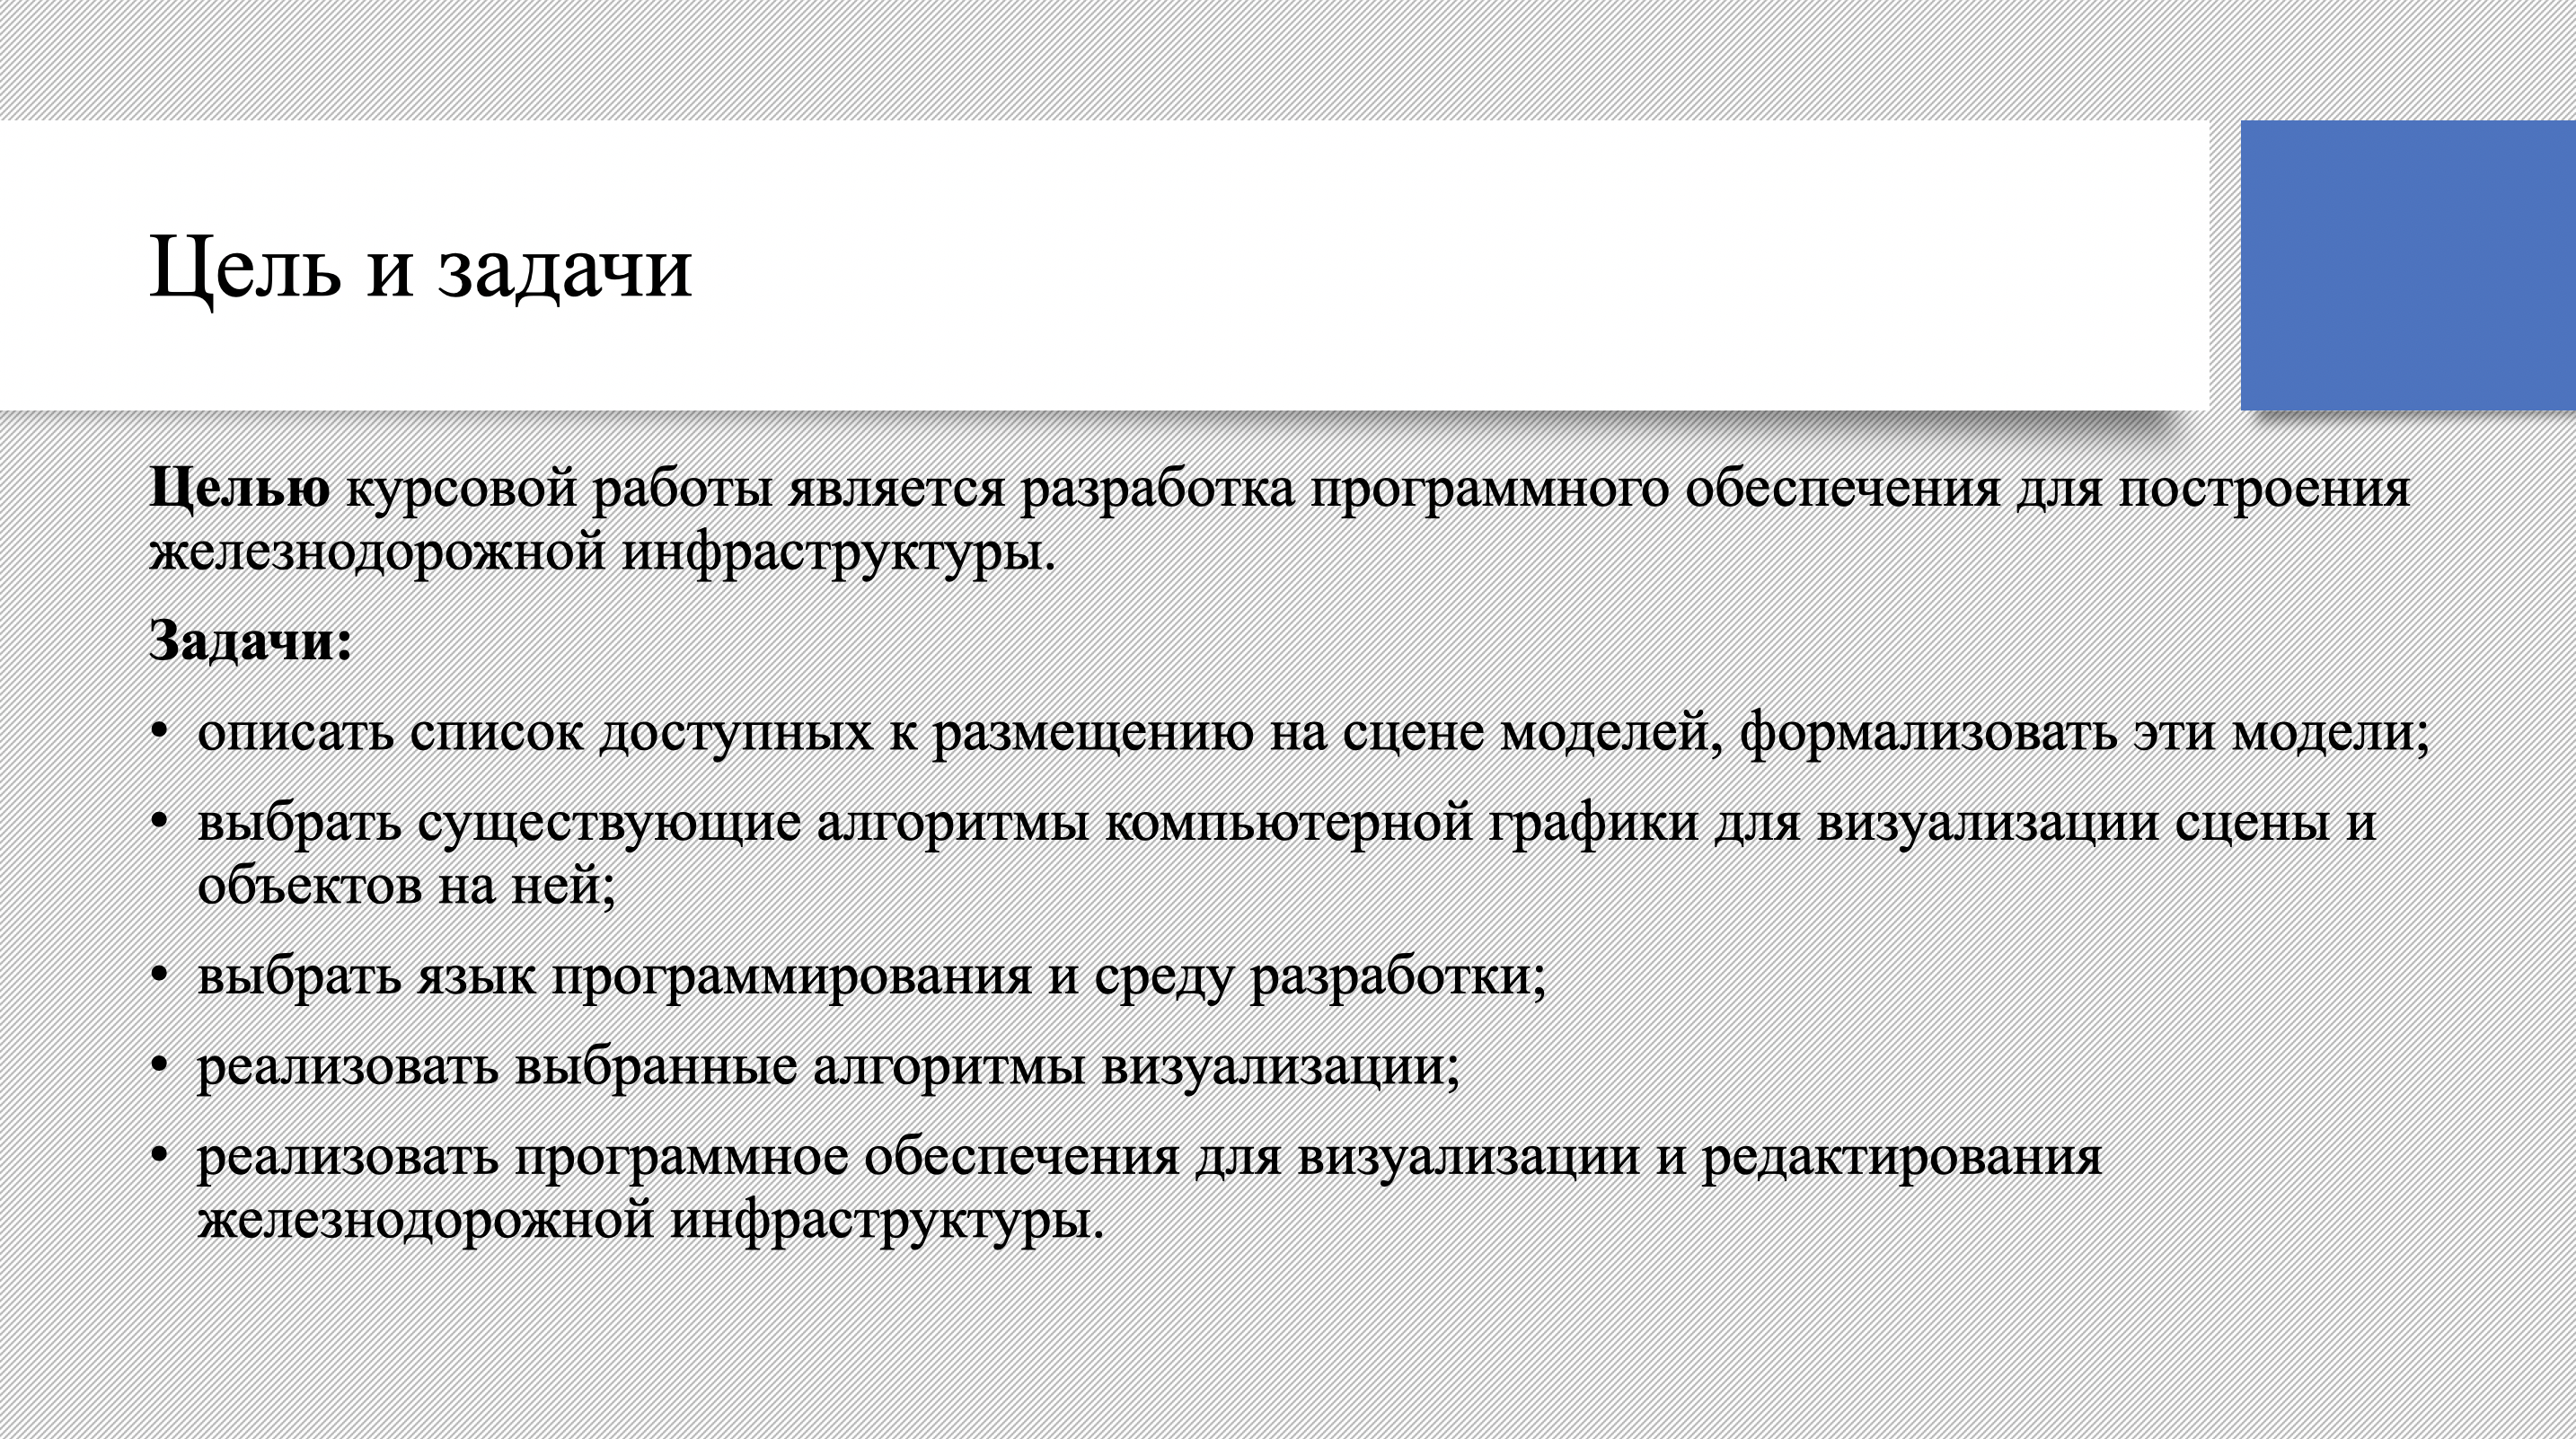
\includegraphics[width=0.5\linewidth]{img/celtask.png}
    \caption{Цели и задачи (слайд 2)}
    \label{img:celtask}
\end{figure}
\noindent

\begin{figure}[h]
    \centering
    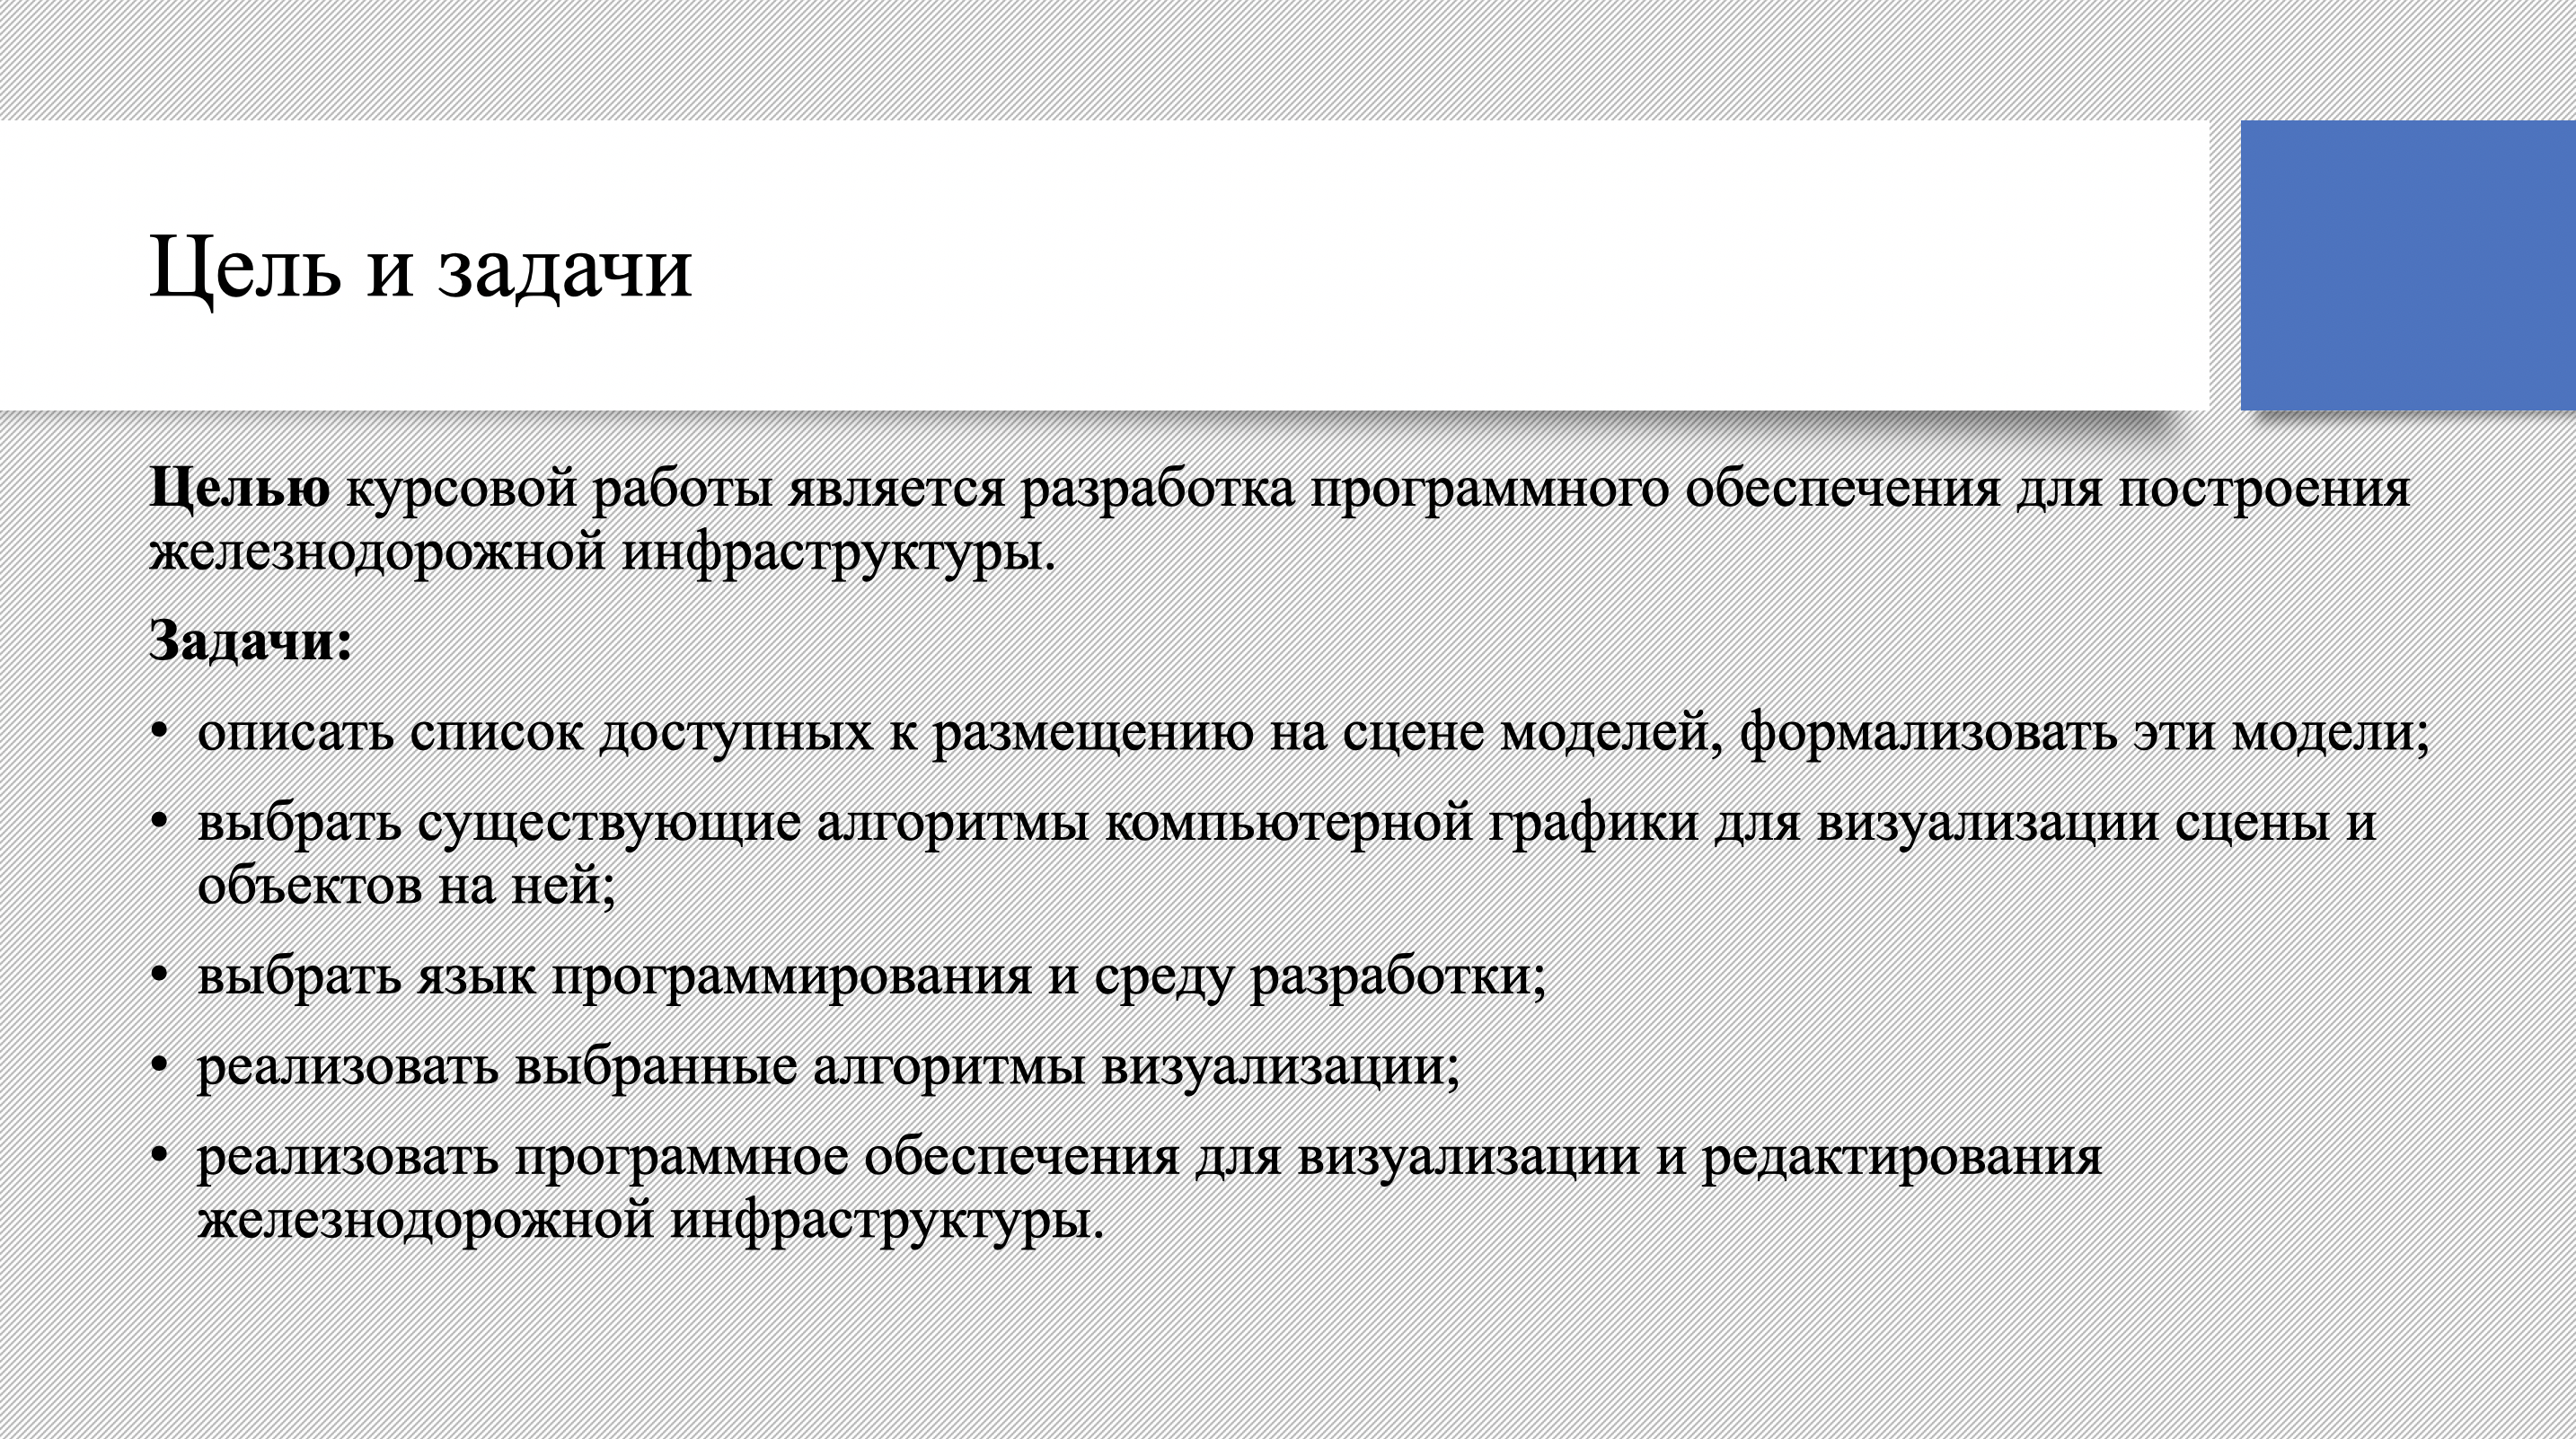
\includegraphics[width=0.5\linewidth]{img/celtask.png}
    \caption{Цели и задачи (слайд 2)}
    \label{img:celtask}
\end{figure}
\noindent

\begin{figure}[h]
    \centering
    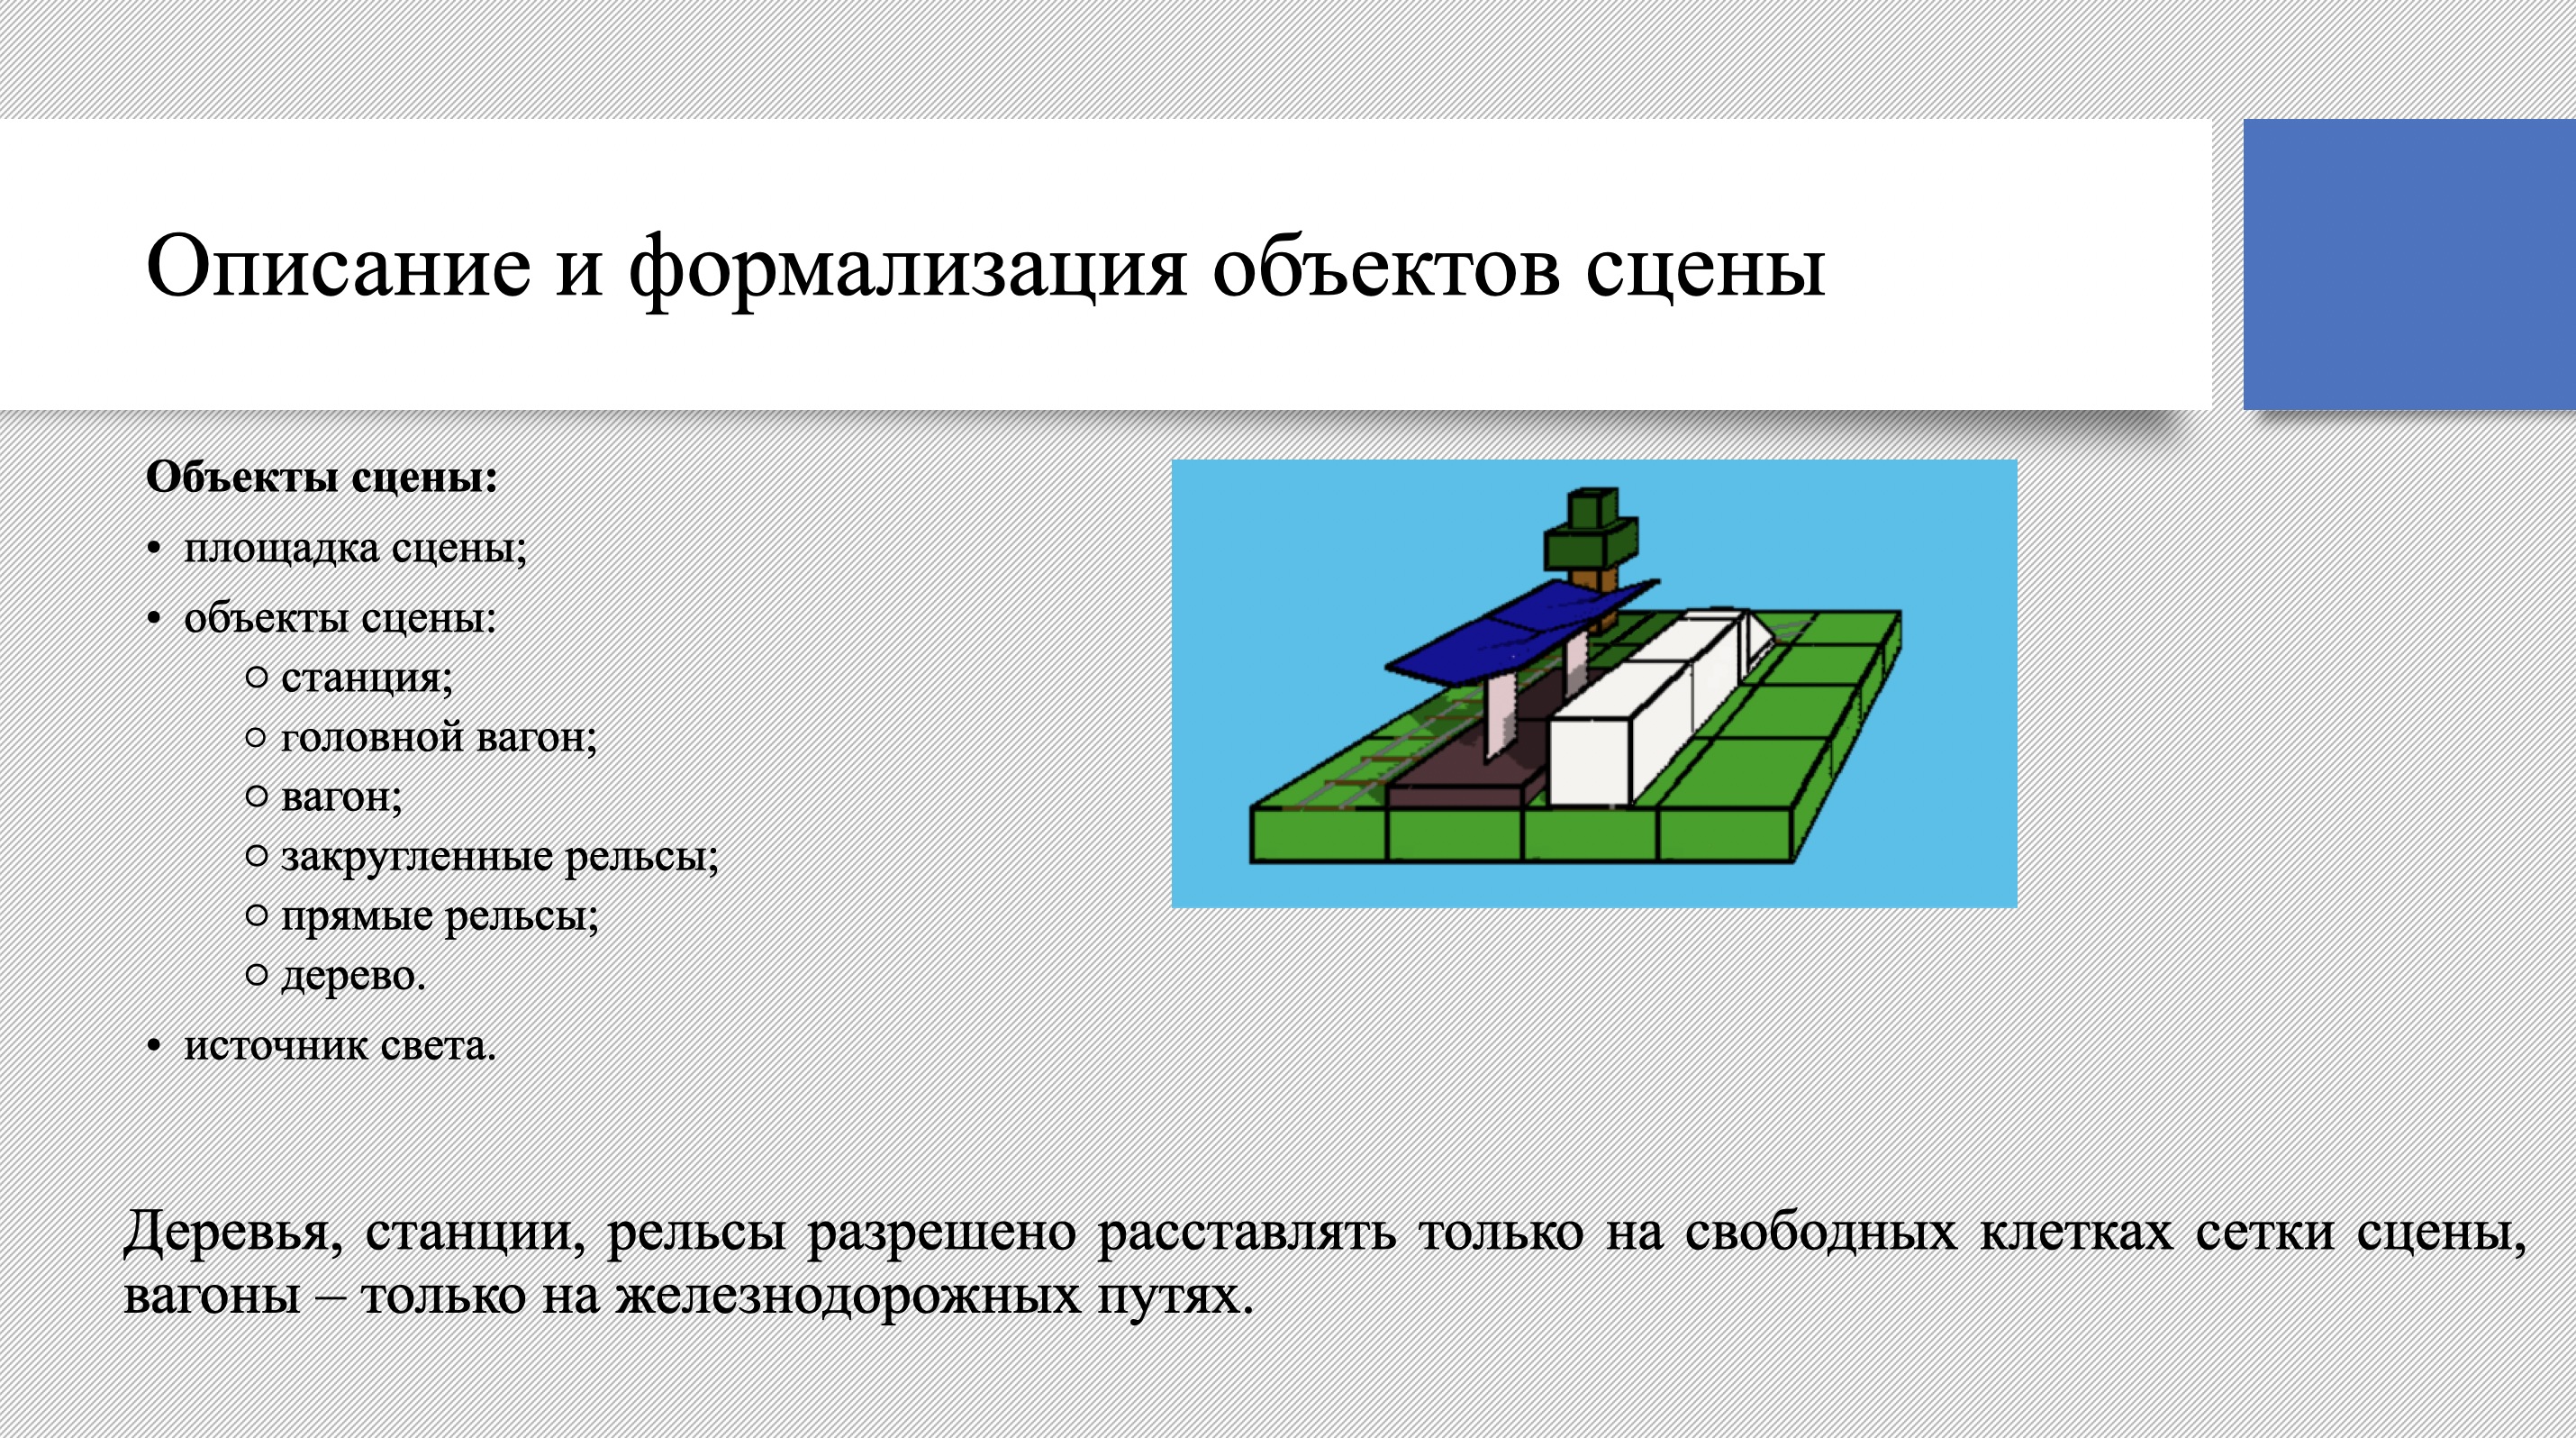
\includegraphics[width=0.5\linewidth]{img/form.png}
    \caption{Описание и формализация объектов сцены (слайд 3)}
    \label{img:form}
\end{figure}
\noindent

\begin{figure}[h]
    \centering
    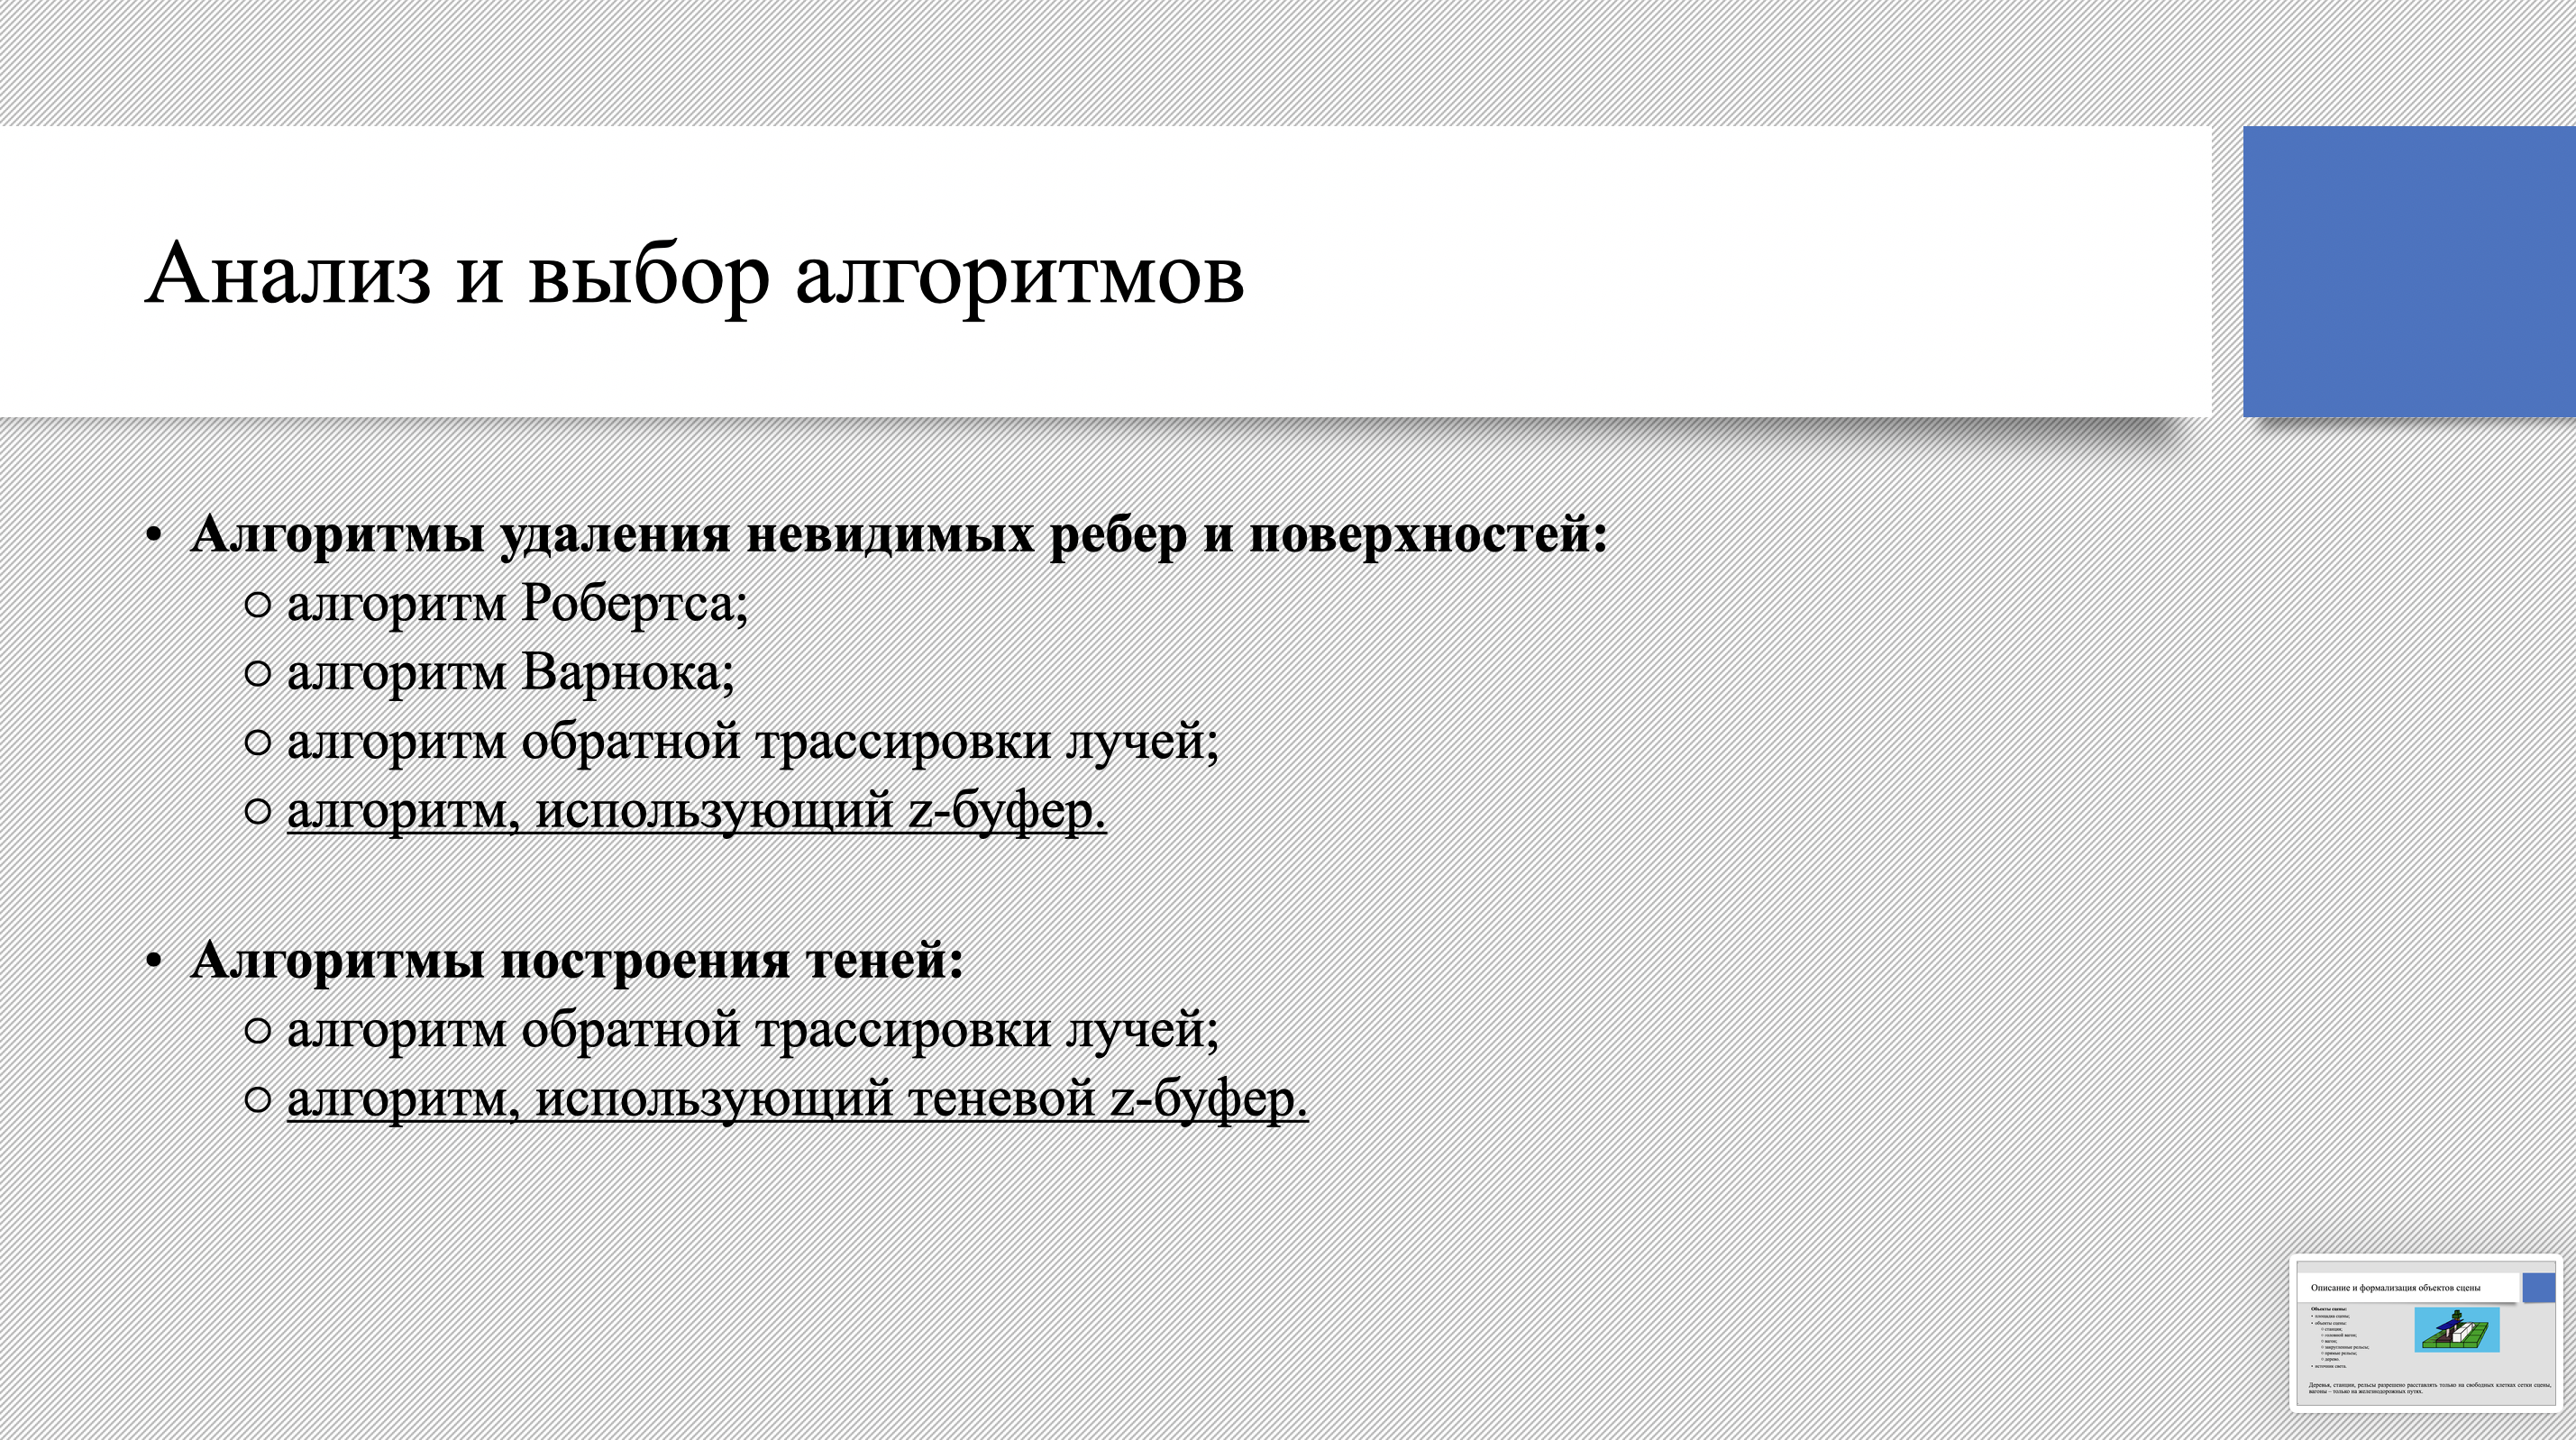
\includegraphics[width=0.5\linewidth]{img/anal.png}
    \caption{Анализ и выбор алгоритмов (слайд 4)}
    \label{img:anal}
\end{figure}
\noindent

\begin{figure}[h]
    \centering
    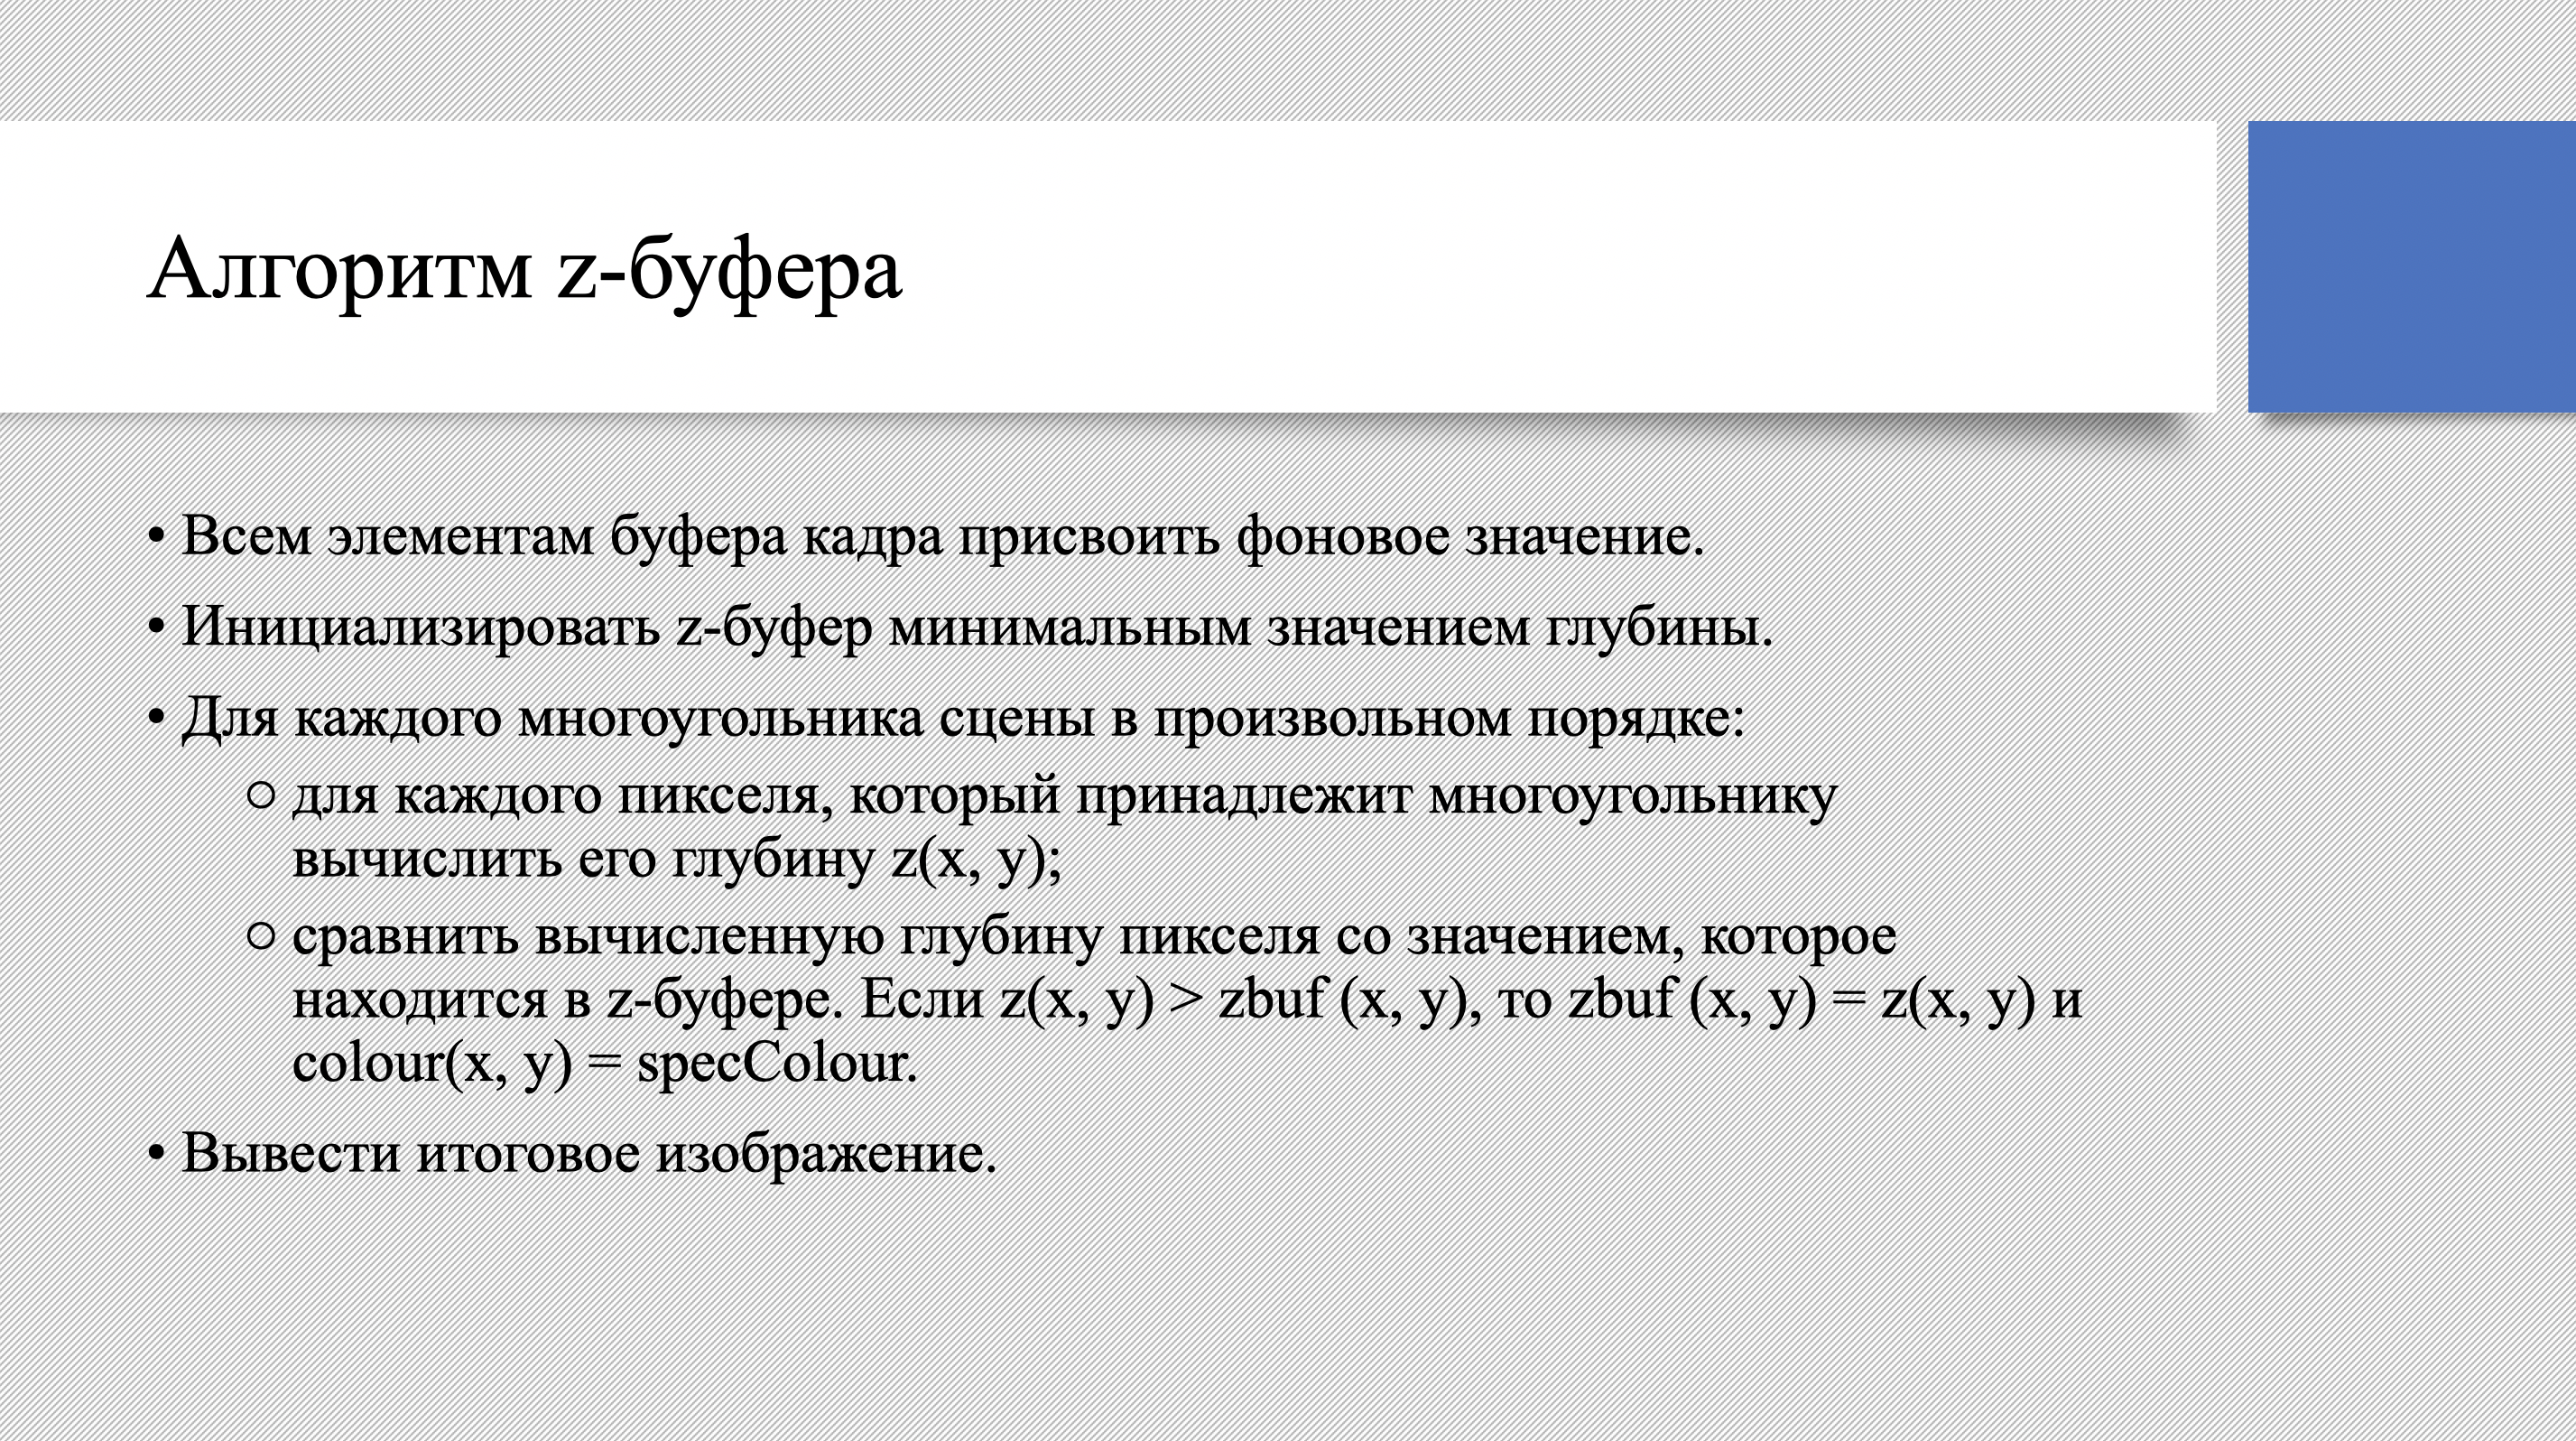
\includegraphics[width=0.5\linewidth]{img/z-buf.png}
    \caption{Анализ z-буфера (слайд 5)}
    \label{img:buf}
\end{figure}
\noindent

\begin{figure}[h]
    \centering
    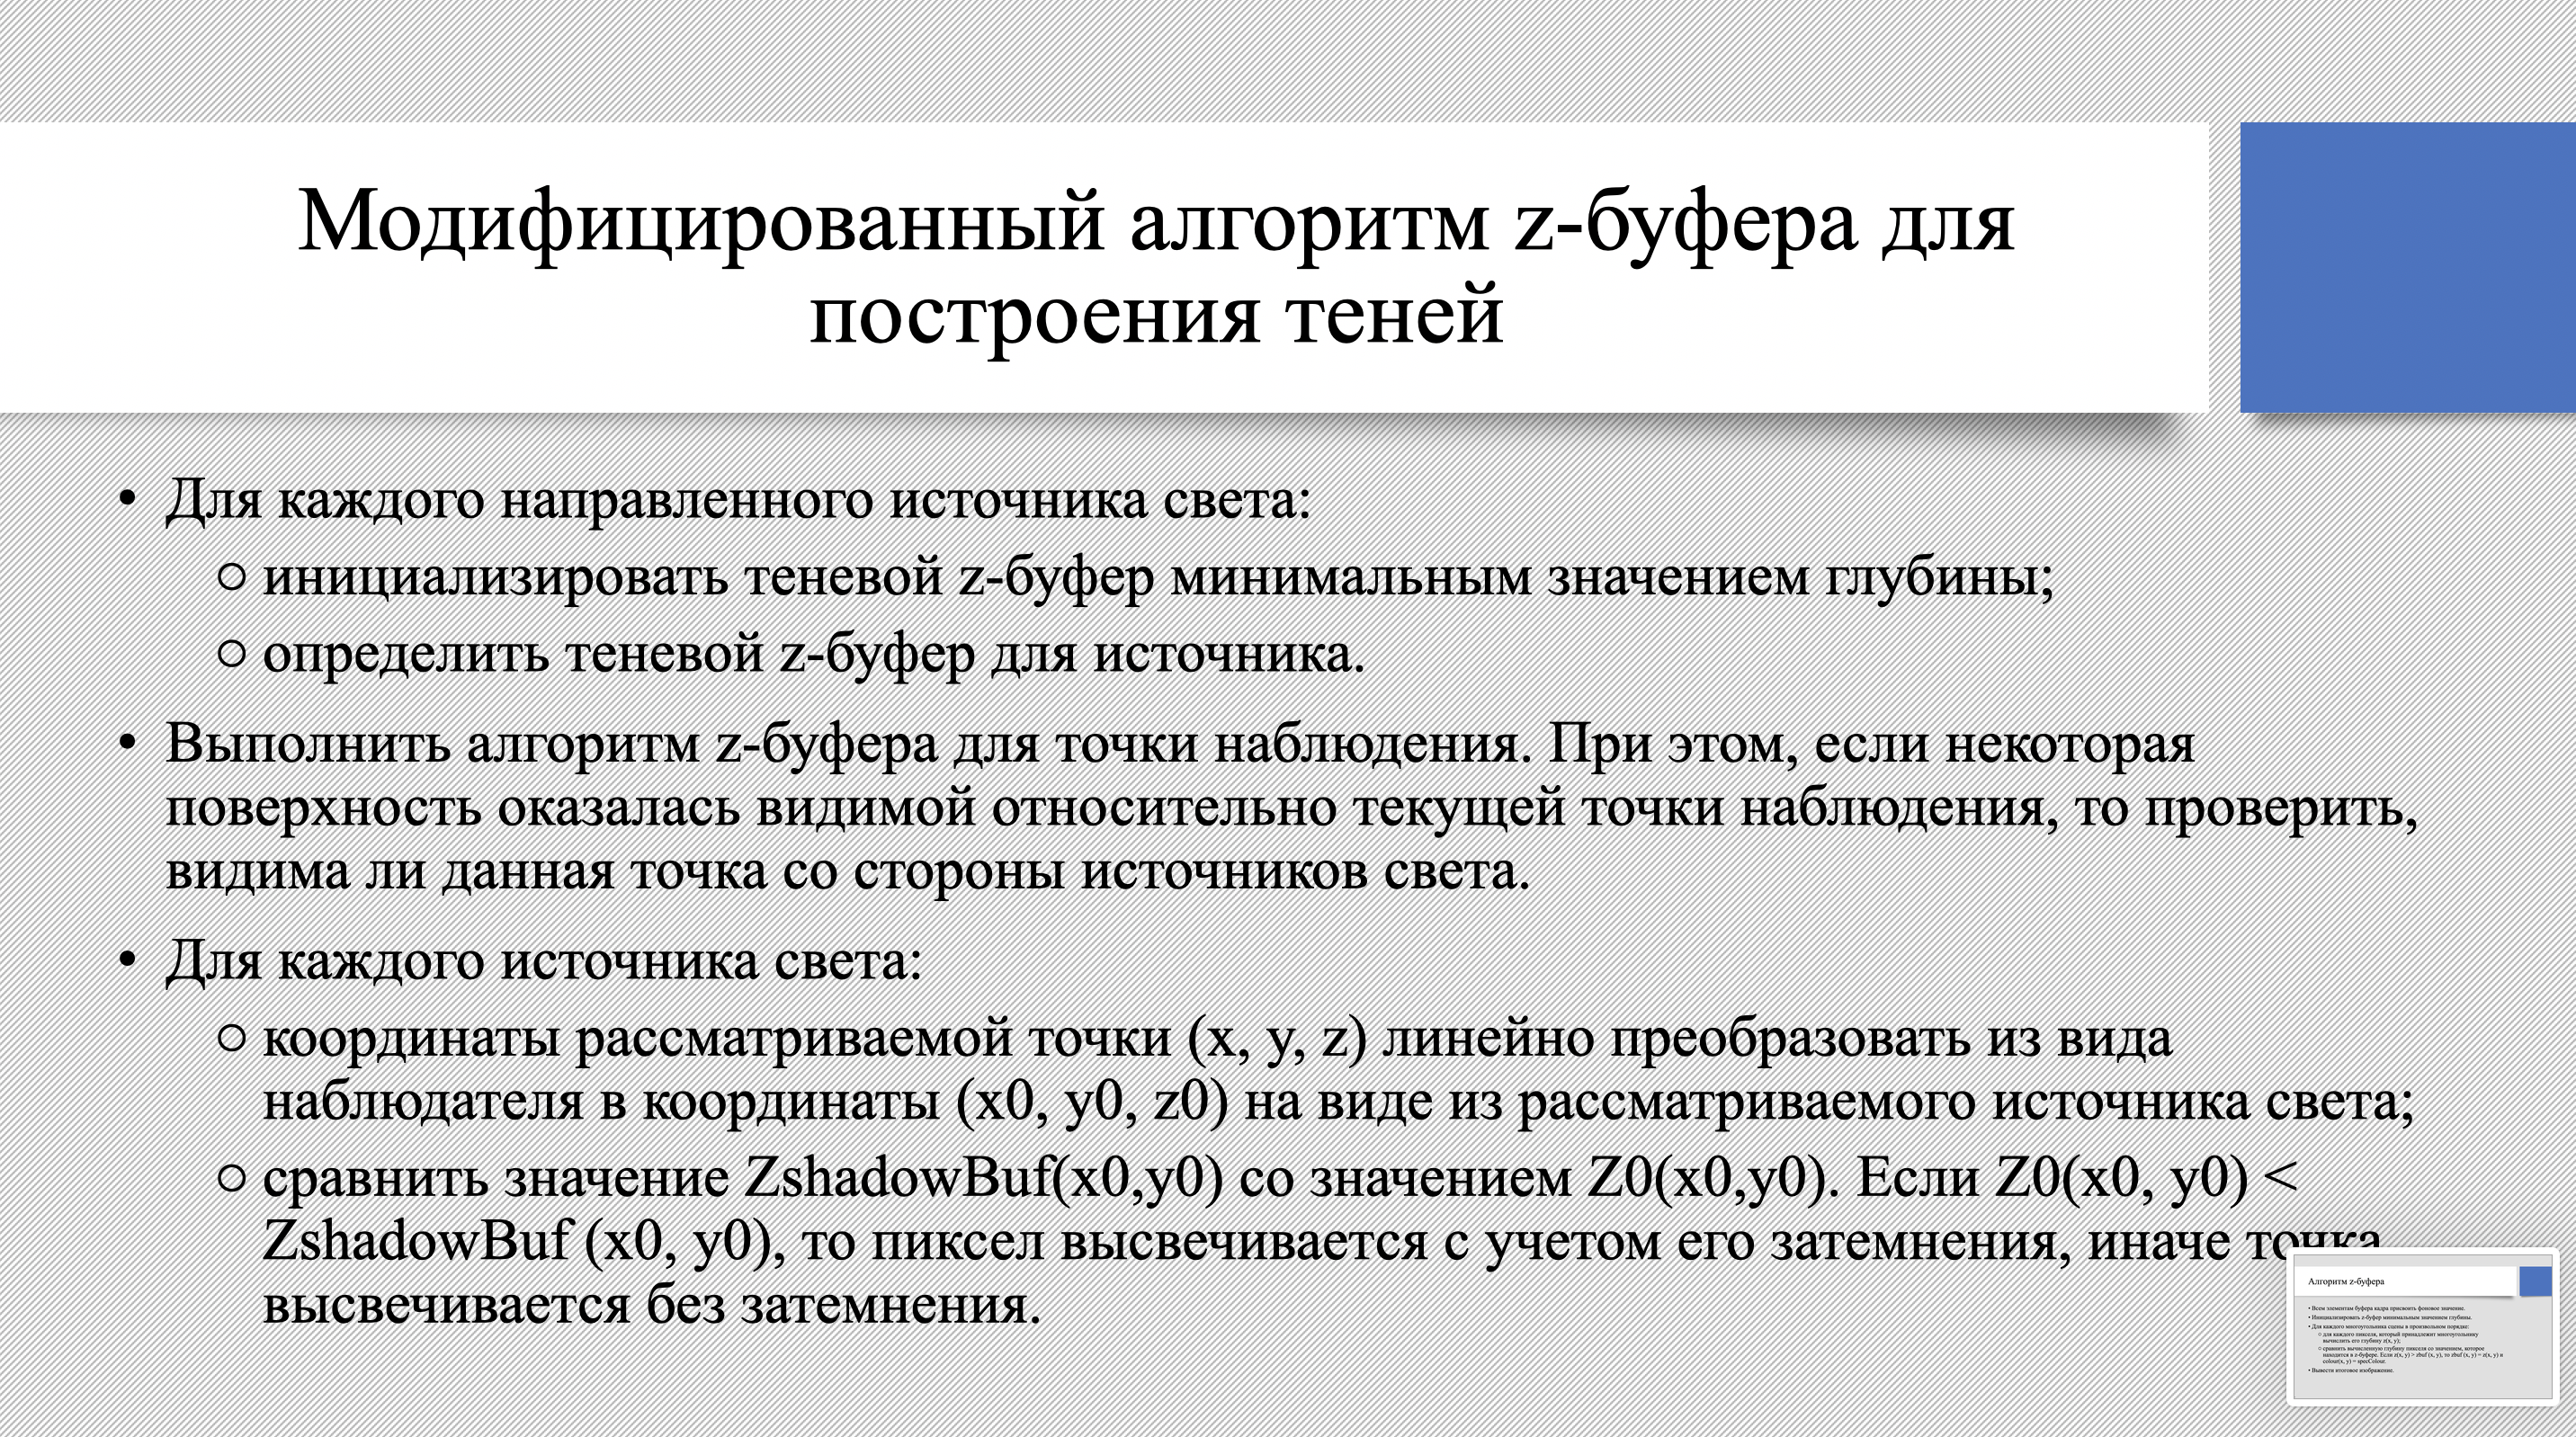
\includegraphics[width=0.5\linewidth]{img/modif.png}
    \caption{Модифицированный алгоритм z-буфера для построения теней (слайд 6)}
    \label{img:modif}
\end{figure}
\noindent

\begin{figure}[h]
    \centering
    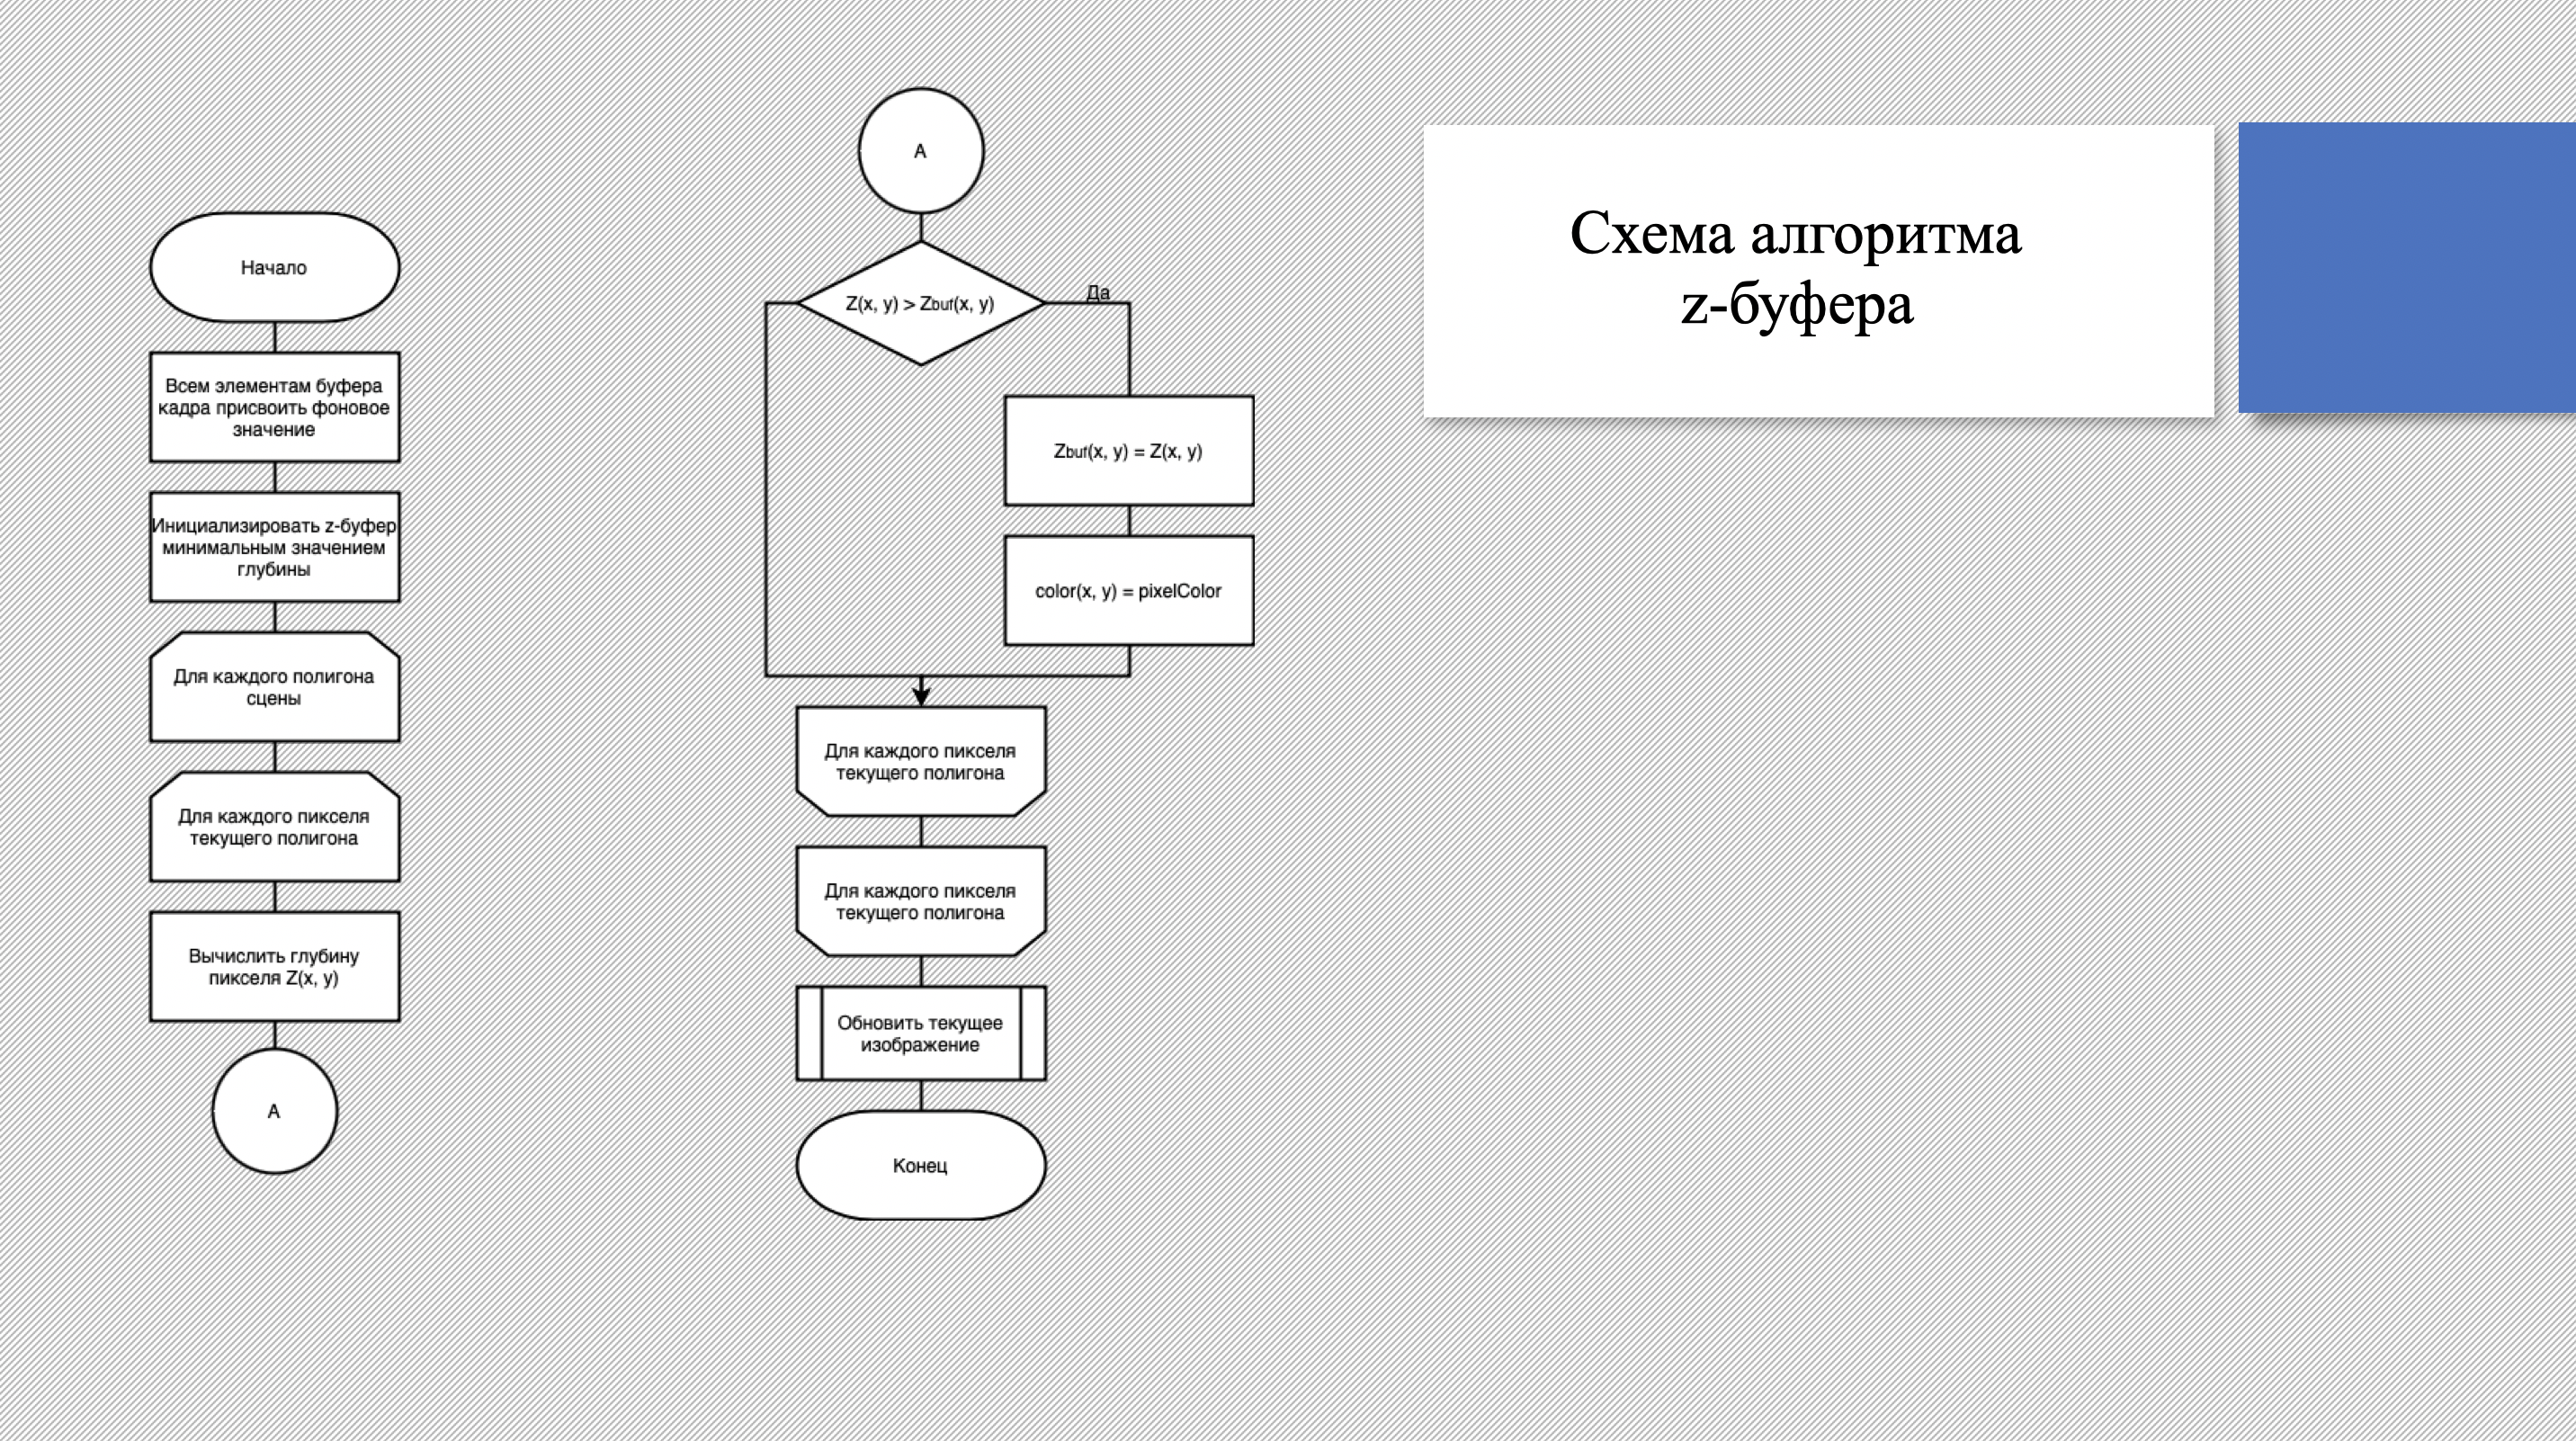
\includegraphics[width=0.5\linewidth]{img/Z.png}
    \caption{Схема алгоритма z-буфера (слайд 7)}
    \label{img:z}
\end{figure}
\noindent

\begin{figure}[h]
    \centering
    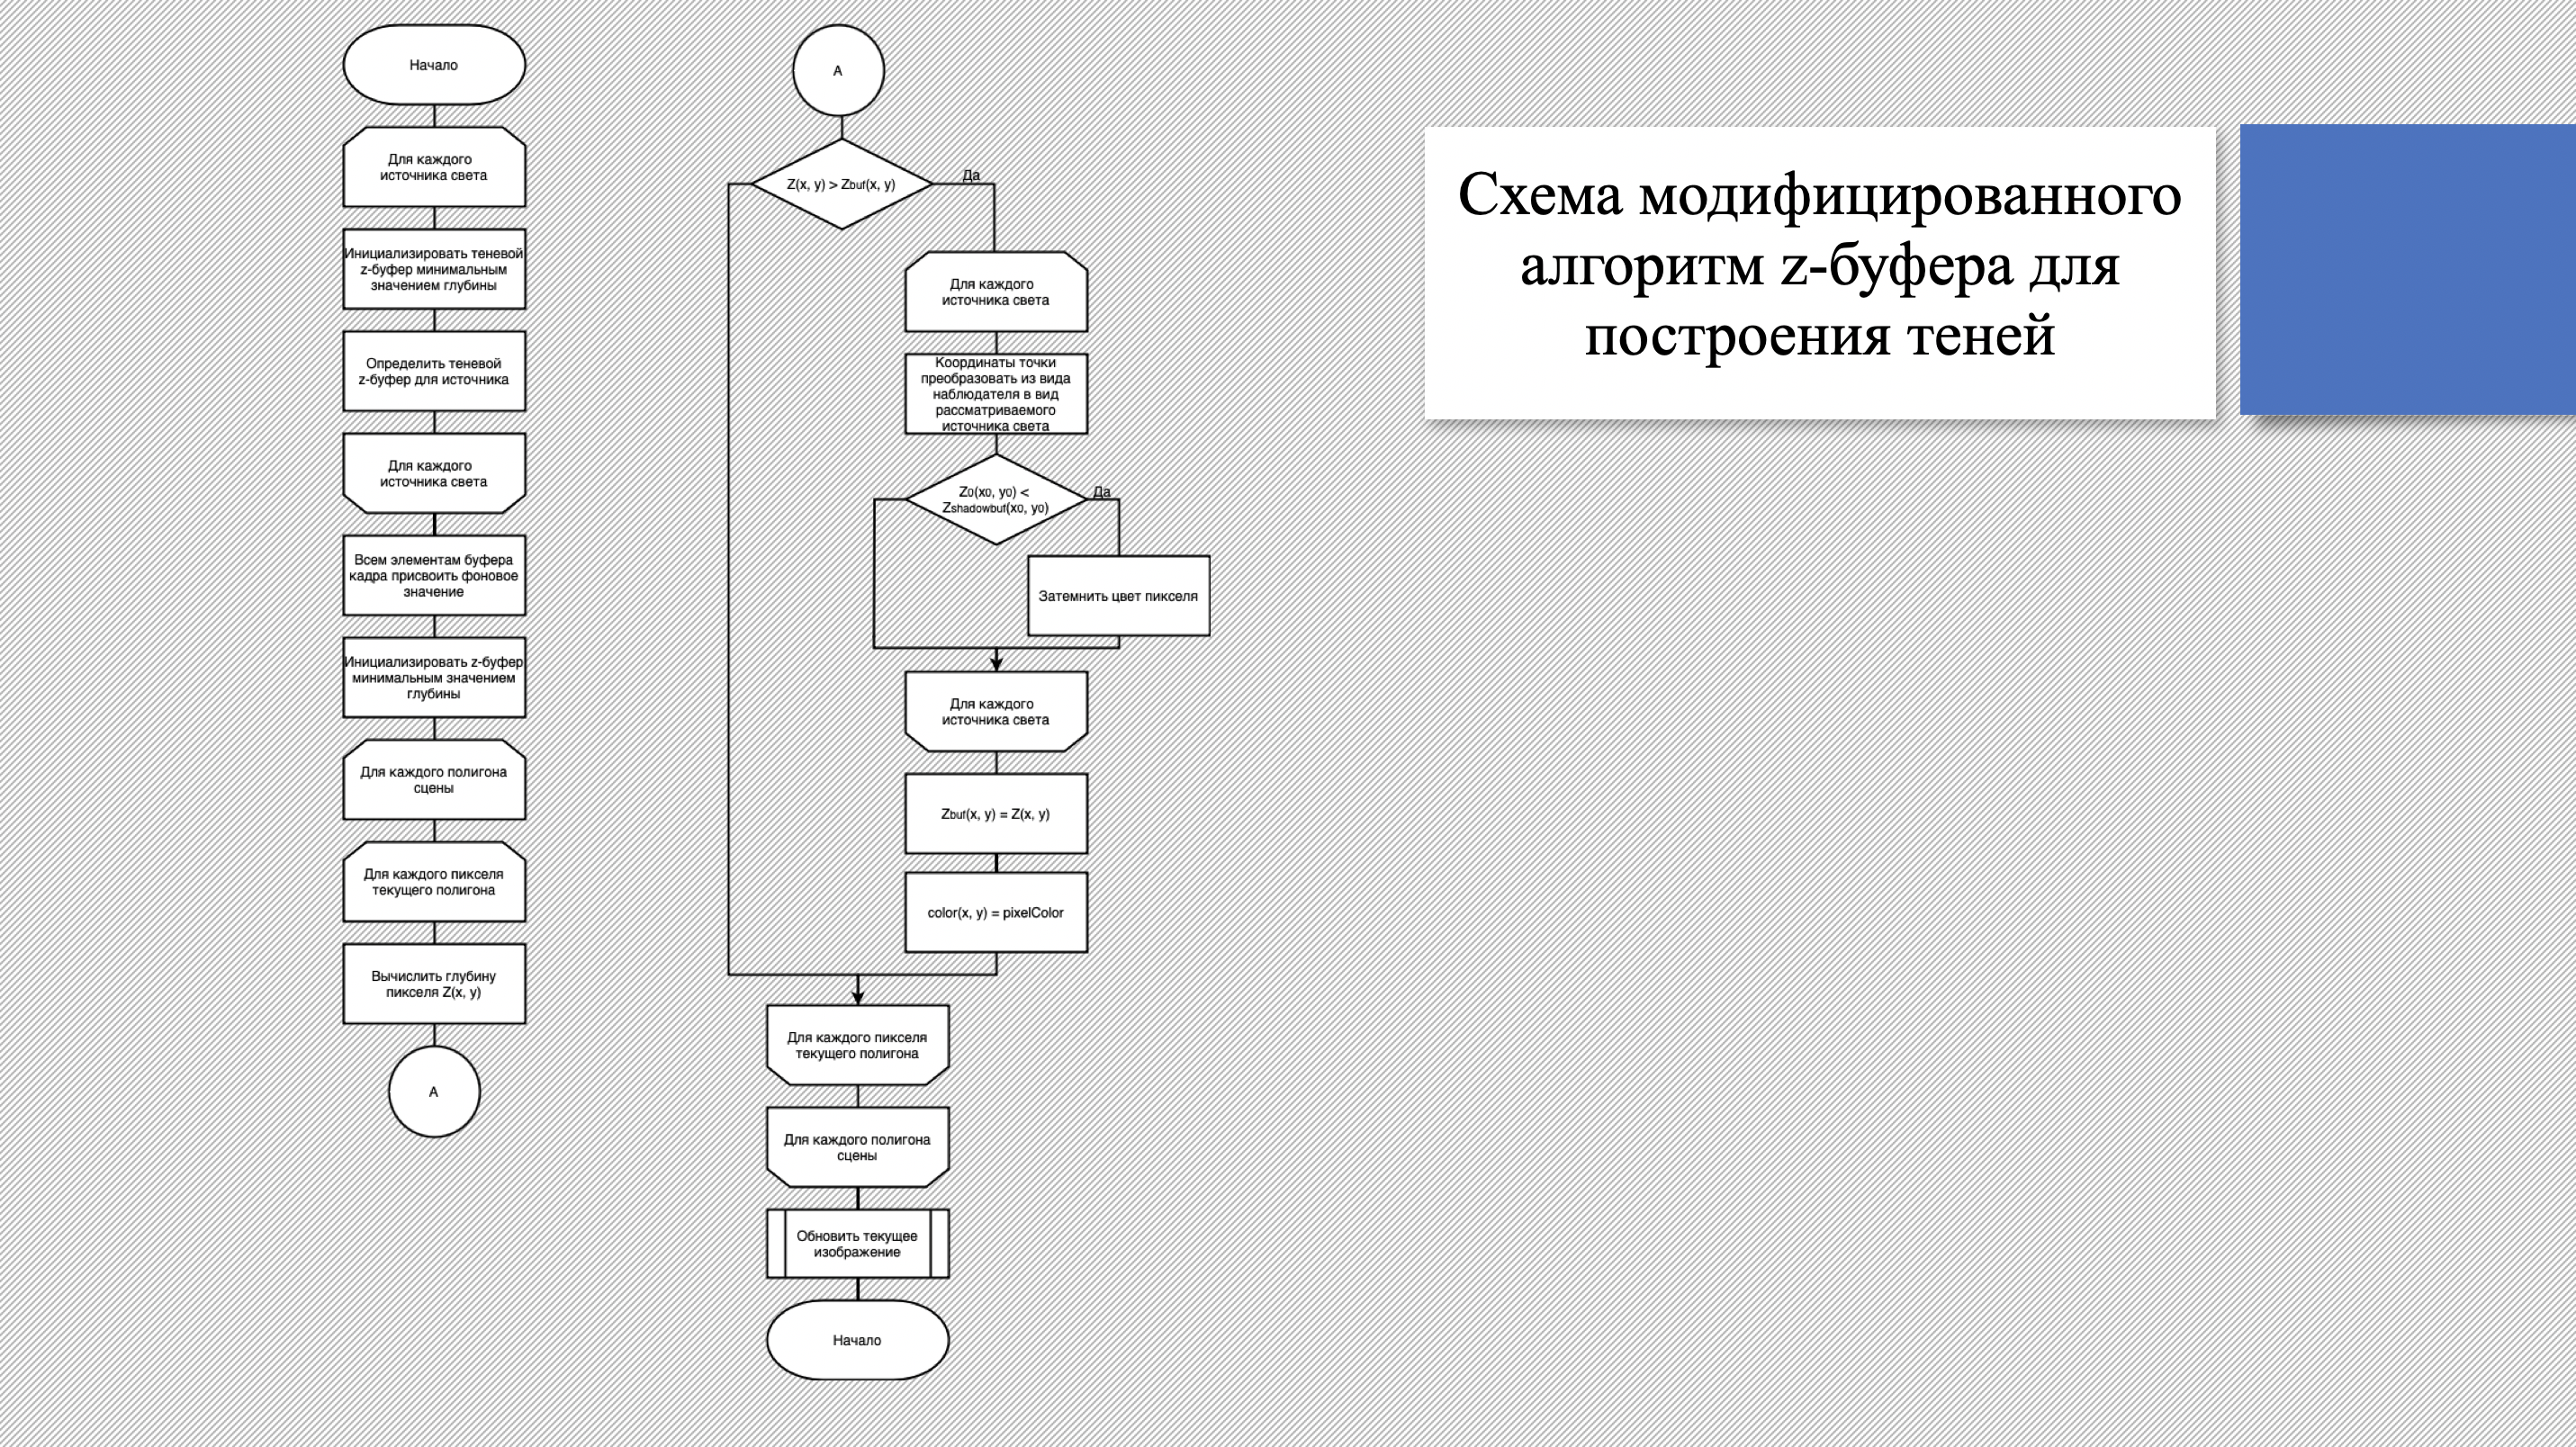
\includegraphics[width=0.5\linewidth]{img/shadow.png}
    \caption{Схема модифицированного алгоритм z-буфера для 
    построения теней (слайд 8)}
    \label{img:shadow}
\end{figure}
\noindent

\begin{figure}[h]
    \centering
    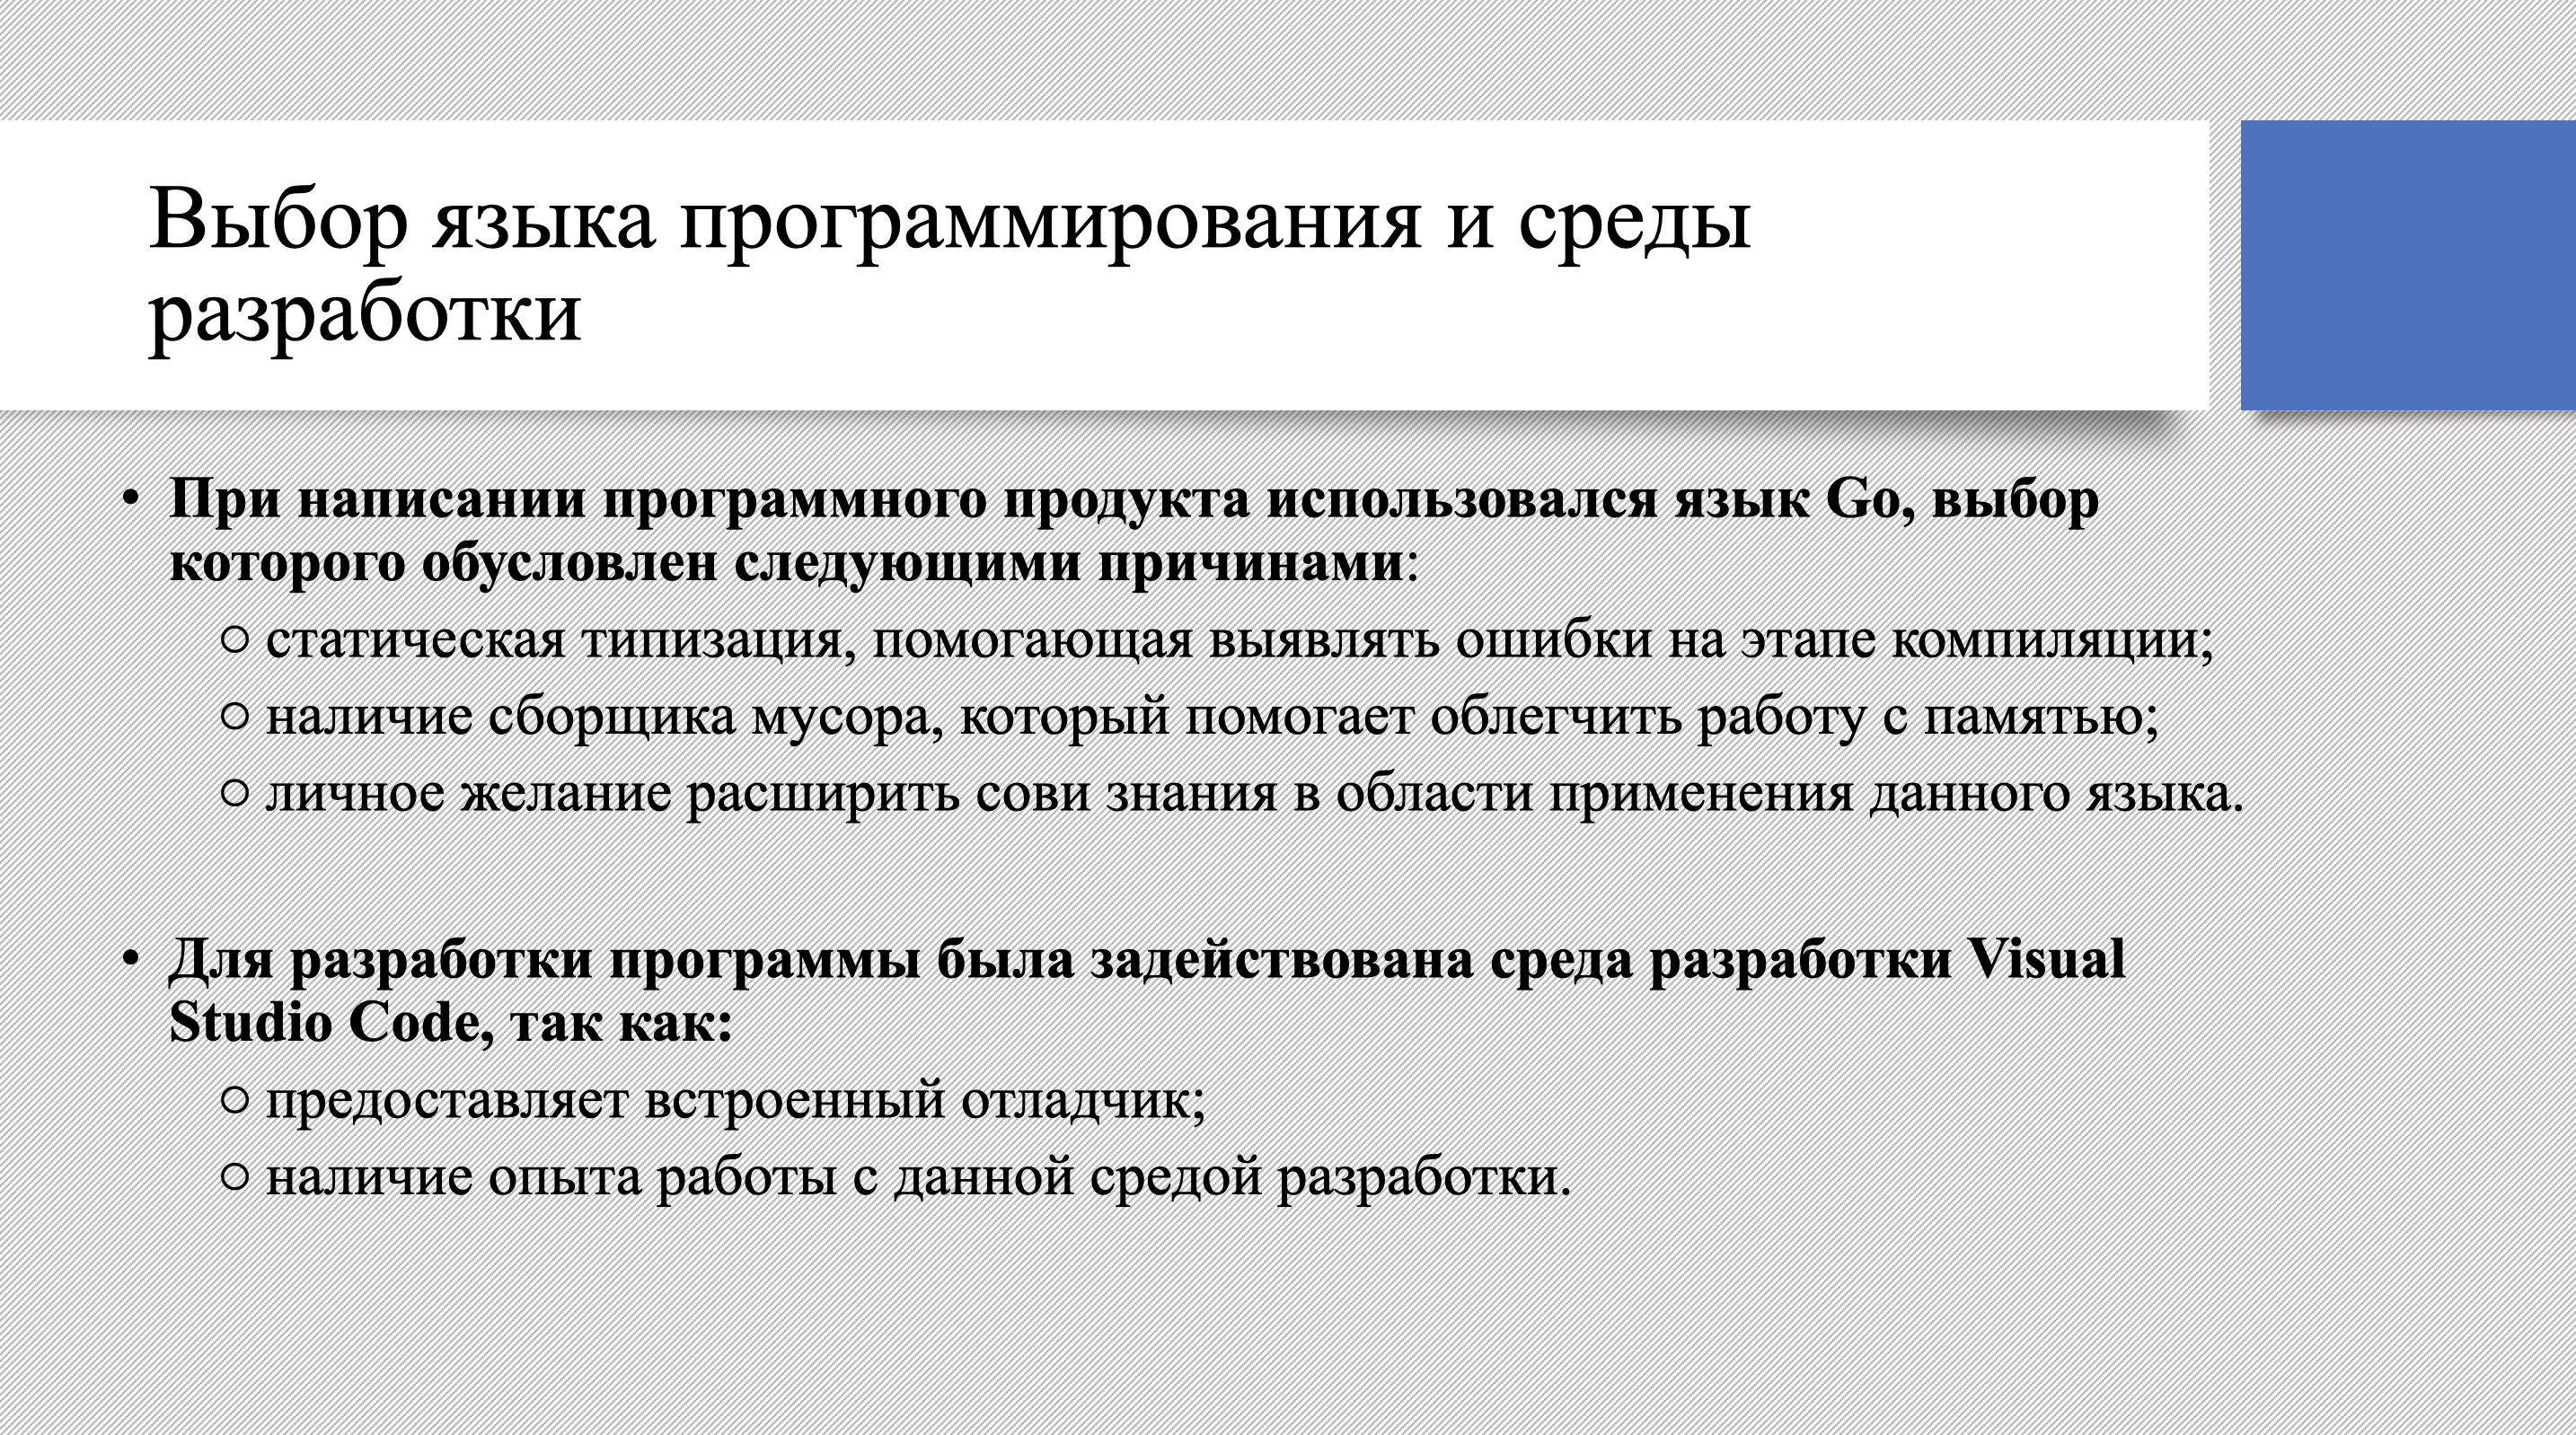
\includegraphics[width=0.5\linewidth]{img/sl.png}
    \caption{Выбор языка программирования и среды разработки (слайд 9)}
    \label{img:sl}
\end{figure}
\noindent

\begin{figure}[h]
    \centering
    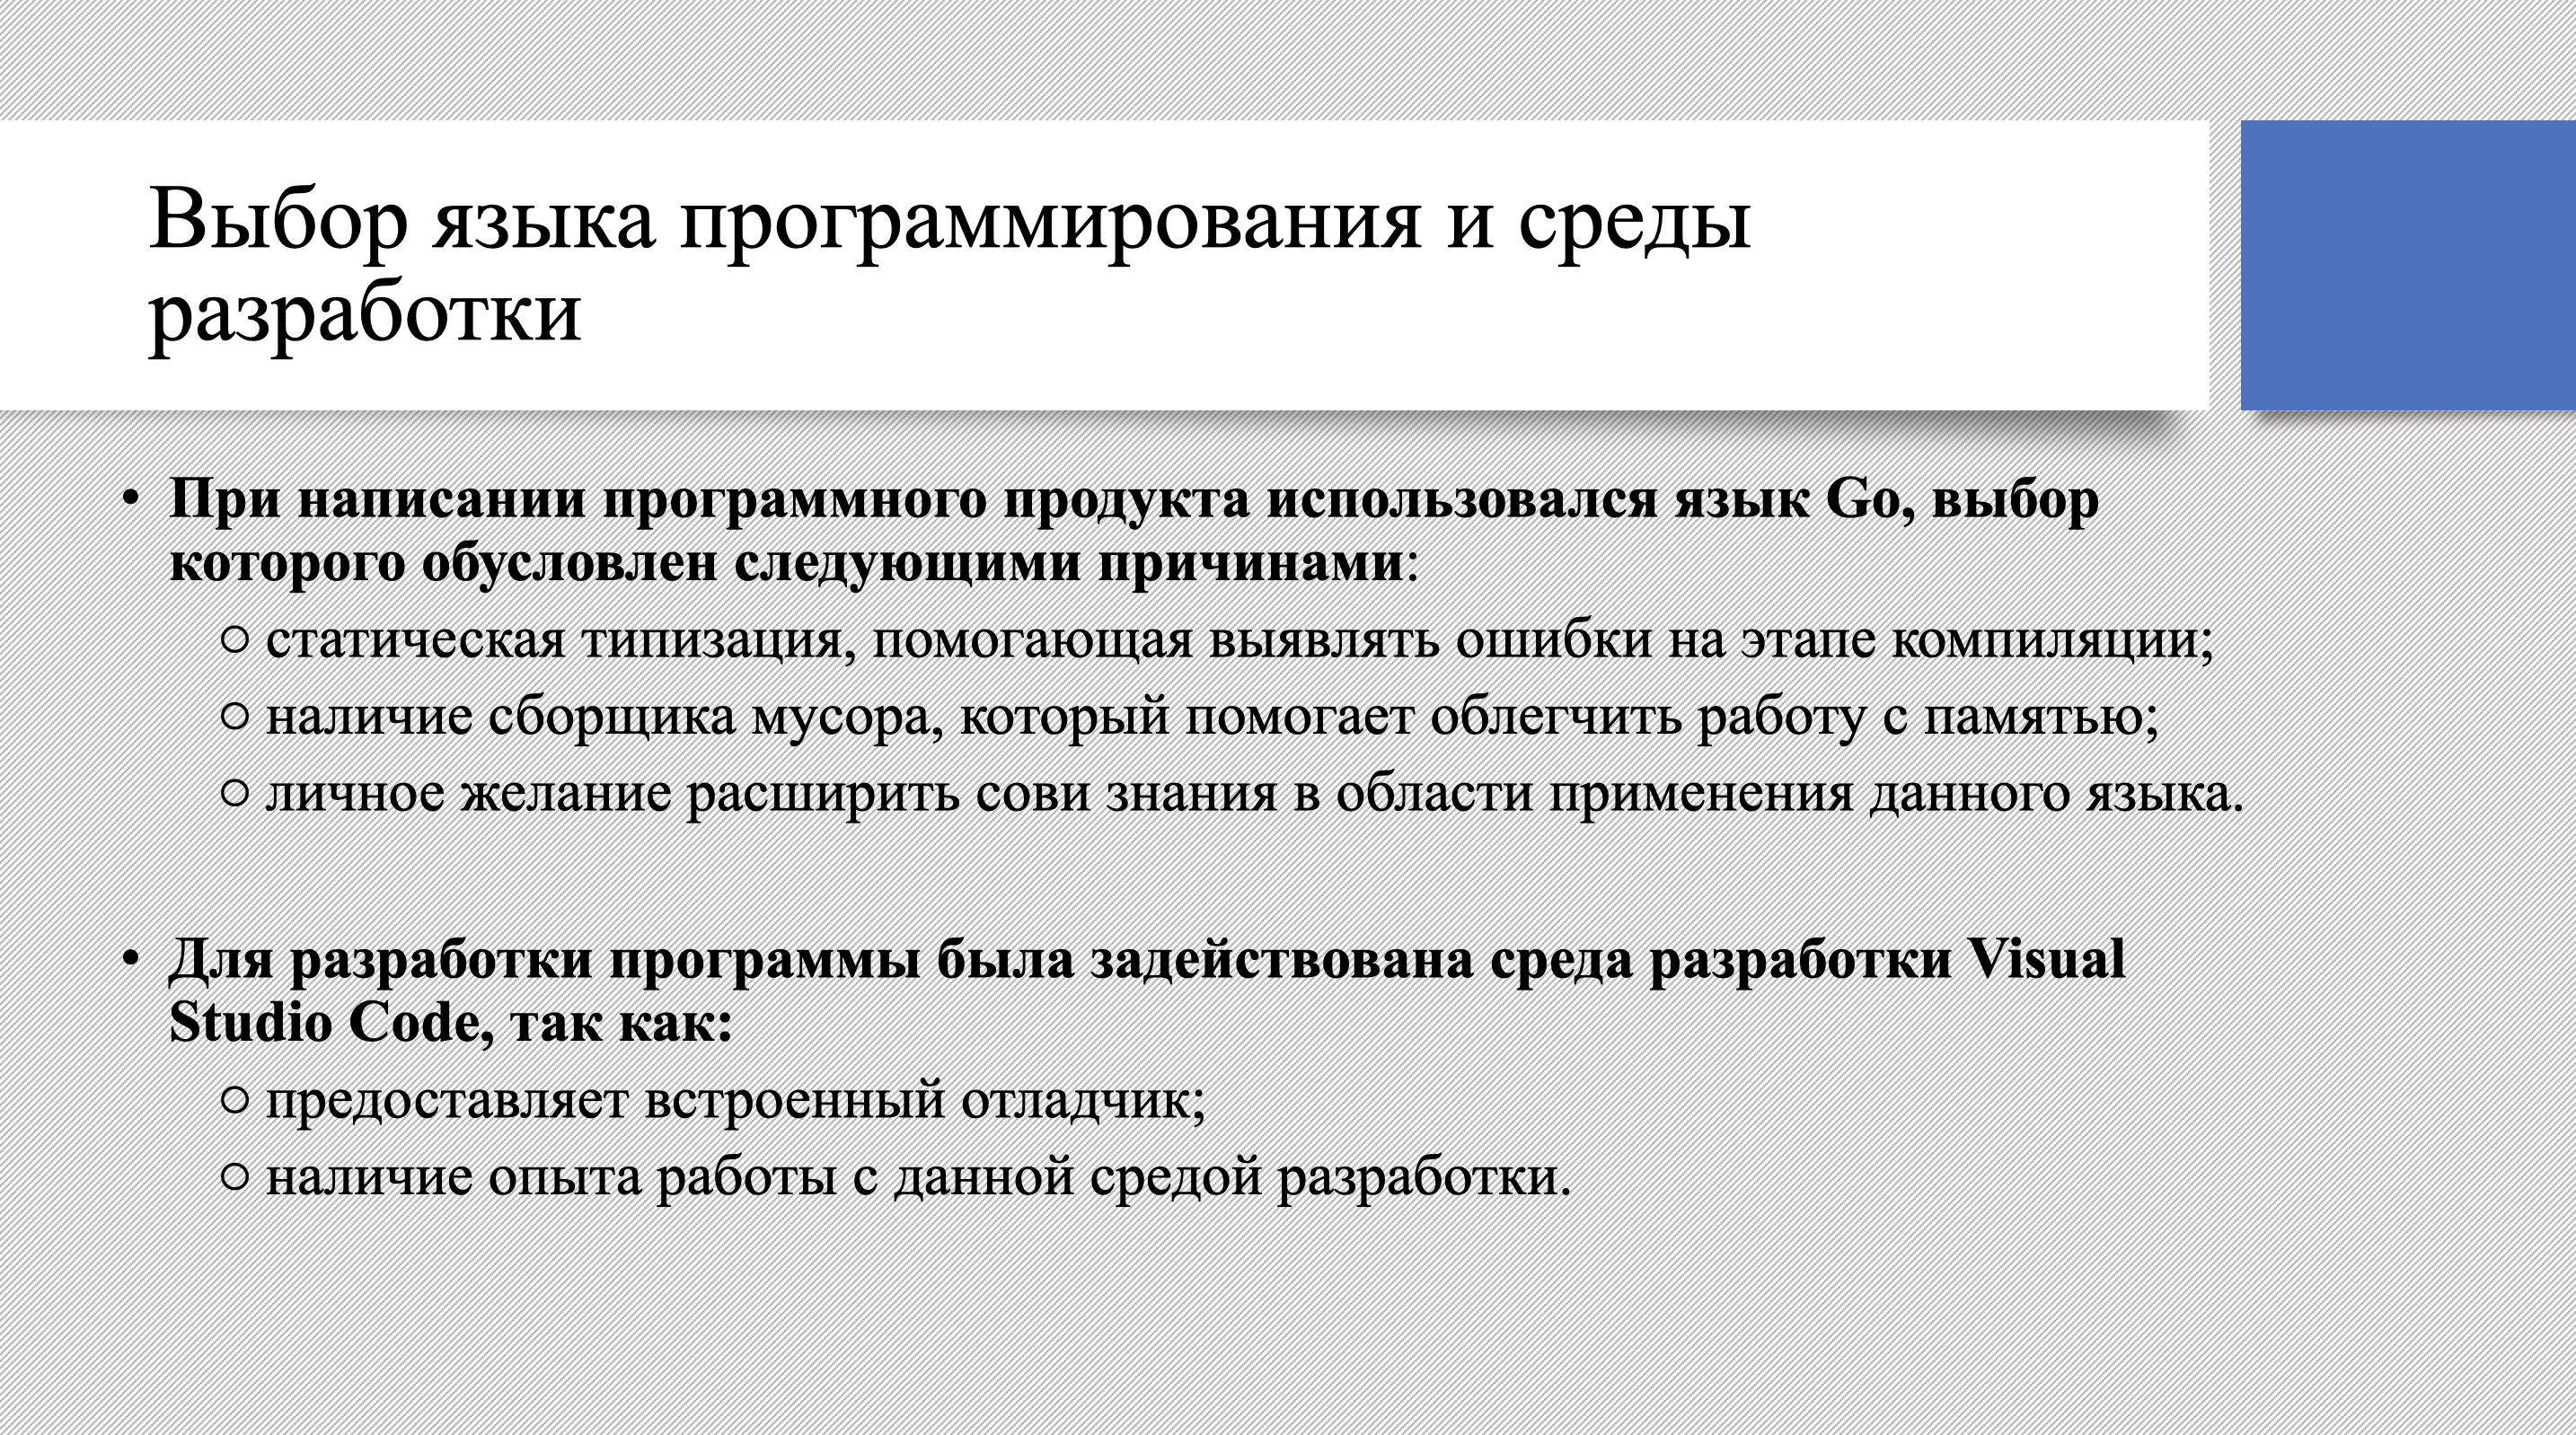
\includegraphics[width=0.5\linewidth]{img/sl.png}
    \caption{Выбор языка программирования и среды разработки (слайд 9)}
    \label{img:sl}
\end{figure}
\noindent

